
%% ============================================================================
%%  Paper presentation: Highly Accurate Protein Structure Prediction with
%%  AlphaFold (Jumper et al., Nature 2021), for Machine Learning for Genomics.
%%  Evita Bosch Pokunevich and Ben Bullinger. Self-contained: the default beamer
%%  theme with three colours and two templates set below.
%%
%%  Build:   latexmk -pdf slides.tex
%%  Figures are cut from the papers: _AF2.pdf, _AF2-SI.pdf, AF3.pdf, by page and trim.
%% ============================================================================
\documentclass[11pt,aspectratio=169]{beamer}

% Theme: beamer's default, stripped. Black headlines, two colours: blue marks the one
% highlighted statement of a slide, red marks what to look at in a figure.
\usetheme{default}
\usefonttheme{professionalfonts}   % beamer leaves the maths fonts to newtxmath
\setbeamertemplate{navigation symbols}{}
\usepackage[T1]{fontenc}
\usepackage{tgheros}   % the sans of the labels drawn on figures
\usepackage{tikz,xcolor,ifthen}
\usepackage{amsmath,amssymb,amsthm,mathtools}   % before newtxmath, which redefines the symbols
\definecolor{ETHBlue}{RGB}{33,92,175}
\definecolor{ETHRed}{RGB}{183,53,45}
\definecolor{ETHGray}{RGB}{111,111,111}
\setbeamercolor*{frametitle}{fg=black}
\setbeamercolor*{item}{fg=black}
\setbeamercolor*{section in toc}{fg=black}
\setbeamerfont{alerted text}{series=\bfseries}
\setbeamertemplate{items}[circle]
\setbeamertemplate{section in toc}[sections numbered]
\setbeamerfont{section in toc}{size=\normalsize}
\newcommand{\tocframe}{
  \begin{frame}[noframenumbering]\frametitle{Outline}\tableofcontents
\end{frame}}
% Serif text (XCharter, close to Nature's Harding) with matching math. Labels drawn on
% figures stay sans, as in the paper's figures.
\usepackage{XCharter}
\usepackage[xcharter,vvarbb]{newtxmath}
\usefonttheme{serif}
\usepackage{bm}   % after newtxmath, or it runs out of math alphabets
\setbeamerfont{frametitle}{family=\rmfamily,size=\Large,series=\bfseries}
\colorlet{accentcolor}{ETHBlue}
\setbeamercolor{alerted text}{fg=accentcolor}
\setbeamerfont{frametitle}{size=\Large}
\setbeamerfont{normal text}{size=\normalsize}
% Frame title, with the subtitle in grey below it when a frame has one. The architecture
% slides use the subtitle for the fact of slide 6 that they answer.
\makeatletter
\setbeamertemplate{frametitle}{\vspace{2mm}\insertframetitle\par
  \ifx\insertframesubtitle\@empty\vspace{4mm}\else
{\vspace{0.5mm}\small\color{ETHGray}\insertframesubtitle\par}\vspace{1.5mm}\fi}
\makeatother

% True footer: citation flushed left, slide number flushed right
\gdef\insertslidecitation{}
\newcommand{\reffootnote}[1]{\gdef\insertslidecitation{#1}}
\newcommand{\slidecitation}[1]{\gdef\insertslidecitation{#1}}
% A citation key in alpha style, [JEP+21]: the first letters of the first three surnames, a plus
% for further authors, the year. The keys are resolved on the reference slides.
\newcommand{\ck}[1]{[#1]}

\newif\ifbackupnumbers   % backup slides are numbered I, II, ... (set after \appendix)
\setbeamertemplate{footline}{%
  \leavevmode%
  \hbox{%
    \begin{beamercolorbox}[wd=\paperwidth,ht=2.8ex,dp=1.2ex,leftskip=1cm,rightskip=1cm]{footline}%
      {\fontsize{5.5pt}{6.5pt}\selectfont\color{ETHGray}\insertslidecitation}%
      \hfill%
      {\fontsize{6.5pt}{7.5pt}\selectfont\color{ETHGray}\ifbackupnumbers\Roman{framenumber}\else\insertframenumber\fi}%
    \end{beamercolorbox}%
  }%
  \gdef\insertslidecitation{}%
}

% Packages
\usepackage{graphicx}
\usepackage{calc}
\usetikzlibrary{arrows.meta,calc}
\usepackage{booktabs,array}
\usepackage{microtype}
\usepackage{pifont}
\usepackage{appendixnumberbeamer}  % backup slides after \appendix do not count in the slide total

\graphicspath{{literature/}}

% Text on a slide: \say{...} is one statement, \key{...} a result or conclusion that the slide
% does not already show. Most slides have none
\newcommand{\say}[1]{{\raggedright #1\par}\vspace{2.5mm}}
\newcommand{\key}[1]{\vspace{1mm}{\raggedright\alert{#1}\par}}

% A figure cut from the paper: page, trim (l b r t), width
\newcommand{\paperfig}[3][0.9\linewidth]{\includegraphics[page=#2,trim=#3,clip,width=#1]{literature/_AF2.pdf}}

% A figure cut from the paper with marks drawn on top: width, page, trim as for \paperfig.
% Inside the environment (0,0) is the lower left corner of the figure and (1,1) the upper right.
\newenvironment{marked}[3][\linewidth]{%
  \begin{tikzpicture}
    \node[anchor=south west, inner sep=0pt] (fig) at (0,0) {\paperfig[#1]{#2}{#3}};
  \begin{scope}[x={(fig.south east)}, y={(fig.north west)}]}%
    {
    \end{scope}
\end{tikzpicture}}
\newenvironment{markedAFthree}[3][\linewidth]{%
  \begin{tikzpicture}
    \node[anchor=south west, inner sep=0pt] (fig) at (0,0)
    {\includegraphics[page=#2,trim=#3,clip,width=#1]{literature/AF3.pdf}};
  \begin{scope}[x={(fig.south east)}, y={(fig.north west)}]}%
    {
    \end{scope}
\end{tikzpicture}}
\newenvironment{markedSI}[3][\linewidth]{%
  \begin{tikzpicture}
    \node[anchor=south west, inner sep=0pt] (fig) at (0,0)
    {\includegraphics[page=#2,trim=#3,clip,width=#1]{literature/_AF2-SI.pdf}};
  \begin{scope}[x={(fig.south east)}, y={(fig.north west)}]}%
    {
    \end{scope}
\end{tikzpicture}}
\tikzset{
  every node/.append style={execute at begin node=\sffamily},
  callout/.style={draw=ETHRed, fill=ETHRed, fill opacity=0.07, line width=0.9pt, rounded corners=1.2pt},  % a frame with a faint tint of its colour
  callout text/.style={text=ETHRed, font=\small, inner sep=1.5pt, text height=1.6ex, text depth=0.4ex},
  cover/.style={fill=white},   % hides a panel letter or a small label of the paper
  cblue/.style={draw=CalloutBlue, fill=CalloutBlue, text=CalloutBlue},
  cpurple/.style={draw=CalloutPurple, fill=CalloutPurple, text=CalloutPurple},
  cgreen/.style={draw=CalloutGreen, fill=CalloutGreen, text=CalloutGreen},
  figure label/.style={font=\footnotesize, inner sep=1.5pt},
}
% Colours of curves and structures in the paper's figures, for legends drawn here
\definecolor{PaperBlue}{RGB}{28,28,205}
\definecolor{PaperGreen}{RGB}{20,170,20}
\definecolor{PaperCurveBlue}{RGB}{25,45,130}
\definecolor{PaperCurveOrange}{RGB}{190,75,25}
\definecolor{PaperCurveGreen}{RGB}{60,140,80}
\definecolor{Gold}{RGB}{204,166,61}
% Callout colours. A box takes the hue of the paper's own box fill, saturated: the paper's pink
% boxes (attention, affinities) get ETH red, its light blue boxes (pair representation, pair
% bias) blue, its lavender boxes (frames, rotation update, outer product mean) purple, its green
% boxes (points, atoms) green. Grey or white figure boxes get red as the neutral highlight.
% A word in the text that refers to a marked part takes the colour of its box: \rd, \bl, \pu, \gn.
\definecolor{CalloutBlue}{RGB}{0,105,170}
\definecolor{CalloutPurple}{RGB}{108,80,170}
\definecolor{CalloutGreen}{RGB}{56,132,74}
\newcommand{\rd}[1]{\textcolor{ETHRed}{#1}}
\newcommand{\bl}[1]{\textcolor{CalloutBlue}{#1}}
\newcommand{\pu}[1]{\textcolor{CalloutPurple}{#1}}
\newcommand{\gn}[1]{\textcolor{CalloutGreen}{#1}}
\colorlet{ipadist}{ETHRed}    % colour of the dashed distances in \ipapair
\colorlet{framecol}{ETHRed}   % colour of the frame triads drawn by \frameaxes
\colorlet{ipaq}{ETHBlue}      % colour of the query points in \ipapair
\newif\ifipalabels\ipalabelstrue  % the short labels i and j in \ipapair; the IPA slide sets its own

% Boxes on the paper's figures. boxes.tex holds the measured extent of every box the slides
% mark, generated by tools/measure_boxes.py from the figure crops. \callbox draws a frame
% with the same padding on every side, so a box is symmetric whatever the crop's aspect ratio.
% \callcircle does the same for a circle, \boxlabel puts a label above, below, left or right.
\newlength{\boxpad}\setlength{\boxpad}{1mm}
\newcommand{\definebox}[5]{\pgfkeyssetvalue{/boxes/#1/x0}{#2}\pgfkeyssetvalue{/boxes/#1/y0}{#3}\pgfkeyssetvalue{/boxes/#1/x1}{#4}\pgfkeyssetvalue{/boxes/#1/y1}{#5}}
\newcommand{\bx}[2]{\pgfkeysvalueof{/boxes/#1/#2}}
\newcommand{\callbox}[2][]{\draw[callout,#1] ([shift={(-\boxpad,-\boxpad)}]\bx{#2}{x0},\bx{#2}{y0}) rectangle ([shift={(\boxpad,\boxpad)}]\bx{#2}{x1},\bx{#2}{y1});}
\newcommand{\callcircle}[2][]{\draw[callout,#1] let \p1=(\bx{#2}{x0},\bx{#2}{y0}), \p2=(\bx{#2}{x1},\bx{#2}{y1}) in ($(\p1)!0.5!(\p2)$) ellipse [x radius={(\x2-\x1)/2+0.6*\boxpad}, y radius={(\y2-\y1)/2+0.6*\boxpad}];}
% \boxlabel[style]{box}{above|below|left|right}{text}
\newcommand{\boxlabel}[4][]{%
  \ifthenelse{\equal{#3}{above}}{\node[callout text,#1, draw=none, fill=none, anchor=south] at ($(\bx{#2}{x0},\bx{#2}{y1})!0.5!(\bx{#2}{x1},\bx{#2}{y1}) + (0,\boxpad+0.5mm)$) {#4};}{}%
  \ifthenelse{\equal{#3}{below}}{\node[callout text,#1, draw=none, fill=none, anchor=north] at ($(\bx{#2}{x0},\bx{#2}{y0})!0.5!(\bx{#2}{x1},\bx{#2}{y0}) - (0,\boxpad+0.5mm)$) {#4};}{}%
  \ifthenelse{\equal{#3}{left}}{\node[callout text,#1, draw=none, fill=none, anchor=east] at ($(\bx{#2}{x0},\bx{#2}{y0})!0.5!(\bx{#2}{x0},\bx{#2}{y1}) - (\boxpad+0.8mm,0)$) {#4};}{}%
\ifthenelse{\equal{#3}{right}}{\node[callout text,#1, draw=none, fill=none, anchor=west] at ($(\bx{#2}{x1},\bx{#2}{y0})!0.5!(\bx{#2}{x1},\bx{#2}{y1}) + (\boxpad+0.8mm,0)$) {#4};}{}}
% Generated by tools/measure_boxes.py from the figure crops. Do not edit by hand.
% \definebox{figure/box}{x0}{y0}{x1}{y1}, fractions of the crop, (0,0) bottom left.
\definebox{fig1e/msa}{0.2380}{0.6901}{0.3486}{1.0000}
\definebox{fig1e/templates}{0.2679}{0.1459}{0.3194}{0.3501}
\definebox{fig1e/evoformer}{0.5303}{0.2564}{0.6075}{0.9652}
\definebox{fig1e/structure}{0.7611}{0.2564}{0.8383}{0.9652}
\definebox{fig1e/recycling}{0.4136}{0.0033}{0.9390}{0.0910}
\definebox{fig1e/output}{0.8796}{0.4846}{0.9649}{0.7028}
\definebox{fig3a/rowatt}{0.1395}{0.5915}{0.1799}{0.8602}
\definebox{fig3a/opm}{0.3734}{0.3869}{0.4155}{0.5674}
\definebox{fig3a/triangles}{0.4322}{0.0316}{0.7488}{0.3502}
\definebox{fig3d/ipa}{0.3467}{0.3331}{0.4342}{0.5592}
\definebox{fig3d/update}{0.4644}{0.2532}{0.6262}{0.3640}
\definebox{fig3d/frames}{0.6498}{0.1153}{0.7973}{0.2540}
\definebox{fig3d/atoms}{0.7707}{0.5411}{0.9324}{0.6647}
\definebox{sfig2/pairbias}{0.3377}{0.0149}{0.4372}{0.2849}
\definebox{sfig2/gating}{0.7257}{0.7106}{0.7530}{0.9760}
\definebox{sfig2/plus}{0.4609}{0.4718}{0.4690}{0.4932}
\definebox{sfig8/pairbias}{0.3825}{0.7049}{0.4619}{0.8388}
\definebox{sfig8/dot}{0.3551}{0.4656}{0.4622}{0.5953}
\definebox{sfig8/sqdist}{0.3548}{0.2309}{0.4619}{0.3522}
\definebox{sfig8/invert}{0.7357}{0.1222}{0.7698}{0.1482}
\definebox{sfig8/plus}{0.4881}{0.5214}{0.4946}{0.5319}
\definebox{sfig9/lowgroup}{0.4026}{0.1451}{0.4678}{0.3516}
\definebox{af3/msa}{0.4125}{0.3707}{0.4703}{0.6395}
\definebox{af3/pairformer}{0.4862}{0.1955}{0.6229}{0.6395}
\definebox{af3/diffusion}{0.7419}{0.1965}{0.8414}{0.5438}


% The thread of the talk at the top right of a slide: the four properties of slide 6 as four
% numbered discs, the ones the slide is about in red. Argument: a comma-separated list of 1 to 4.
\newcommand{\props}[1]{%
  \begin{tikzpicture}[remember picture, overlay]
    \foreach \n in {1,...,3} {
      \coordinate (c) at ([xshift=-1cm-3*5.5mm+\n*5.5mm, yshift=-6mm]current page.north east);
      \draw[ETHGray!50, line width=0.7pt] (c) circle (2.2mm);
      \node[font=\scriptsize\sffamily, text=ETHGray] at (c) {\n};
    }
    \foreach \n in {#1} {
      \coordinate (c) at ([xshift=-1cm-3*5.5mm+\n*5.5mm, yshift=-6mm]current page.north east);
      \fill[ETHRed] (c) circle (2.2mm);
      \node[font=\scriptsize\sffamily\bfseries, text=white] at (c) {\n};
    }
\end{tikzpicture}}

% A frame, as drawn on the slides on IPA and FAPE: a 3D triad seen in isometric view, the
% three axes 120 degrees apart. Arguments: position, rotation of the triad in the plane.
\newcommand{\frameaxes}[2]{%
  \foreach \a in {90,210,330}
  \draw[framecol, line width=1.2pt, -{Latex[length=4pt]}] #1 -- ++(#2+\a:0.72);
  \fill[framecol] #1 circle (2.4pt);
}
% The drawing on the slide on invariant point attention: a short chain, residues i and j
% with their frames, four points each placed in the frame. The dashed lines are the
% distances in the formula. An illustration, not data.
\newcommand{\ipapair}{%
  \draw[ETHGray!40, line width=2.6pt, line join=round, line cap=round]
  (-1.3,-0.7) -- (0,0) -- (1.4,-1.9) -- (2.9,-1.6) -- (3.6,0.1) -- (4.6,1.0);
  \foreach \p in {(-1.3,-0.7), (1.4,-1.9), (2.9,-1.6), (4.6,1.0)} \fill[ETHGray!70] \p circle (2pt);
  \foreach \q/\k in {{(1.0,0.9)}/{(2.5,1.0)}, {(1.3,0.3)}/{(2.25,0.4)}, {(1.2,-0.3)}/{(2.4,-0.25)}, {(0.8,-0.7)}/{(2.65,-0.8)}} {
    \draw[ipaq!45, line width=0.6pt] (0,0) -- \q;
    \draw[black!40, line width=0.6pt] (3.6,0.1) -- \k;
    \draw[ipadist, line width=0.9pt, densely dashed] \q -- \k;
    \fill[ipaq] \q circle (2.4pt);
    \fill[black] \k circle (2.4pt);
  }
  \frameaxes{(0,0)}{20}
  \frameaxes{(3.6,0.1)}{-15}
  \ifipalabels
  \node[font=\small, text=framecol] at (-0.85,0.15) {$T_i$};
  \node[font=\small, text=framecol] at (4.62,-0.5) {$T_j$};
  \fi
}
% The alignment drawn on the MSA slide and on the training slide. An illustration, not real
% data: columns 3 and 9 change together.
\newcommand{\msarows}{%
  {M,T,K,V,L,I,N,G,E,L,A,F},
  {M,S,K,V,L,V,N,G,E,L,A,F},
  {M,T,R,I,L,I,N,G,D,L,A,Y},
  {M,T,E,V,L,I,N,G,K,L,-,F},
  {M,T,E,V,L,I,N,G,K,L,A,Y},
{M,S,D,V,L,I,N,G,R,V,A,F}}
% A formula term with its name underneath
\newcommand{\term}[2]{\underbrace{#1}_{\mbox{\footnotesize #2}}}
% The four drawings on the properties slide, one per property.
% Property 1: three aligned sequences, two columns change together (blue and red swap).
\newcommand{\pictofamily}{
  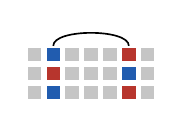
\begin{tikzpicture}[x=1mm, y=1mm, baseline={([yshift=-0.52em]current bounding box.north)}]
    \foreach \r/\ca/\cb in {2.4/ETHBlue/ETHRed, 0/ETHRed/ETHBlue, -2.4/ETHBlue/ETHRed} {
      \foreach \c in {0,...,6} \fill[ETHGray!40] (\c*2.4, \r) ++(-0.85,-0.85) rectangle ++(1.7,1.7);
      \fill[\ca] (2.4, \r) ++(-0.85,-0.85) rectangle ++(1.7,1.7);
      \fill[\cb] (12, \r) ++(-0.85,-0.85) rectangle ++(1.7,1.7);
    }
    \draw[black, line width=0.6pt] (2.4,3.5) .. controls (2.4,5.7) and (12,5.7) .. (12,3.5);
\end{tikzpicture}}
\newcommand{\pictotriangle}{
  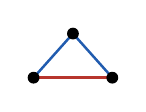
\begin{tikzpicture}[x=1mm, y=1mm, baseline={([yshift=-0.52em]current bounding box.north)}]
    \draw[ETHBlue, line width=0.9pt] (4,-2.6) -- (9,3) -- (14,-2.6);
    \draw[ETHRed, line width=1.3pt] (4,-2.6) -- (14,-2.6);
    \foreach \p in {(4,-2.6),(9,3),(14,-2.6)} \fill[black] \p circle (0.75);
\end{tikzpicture}}
\newcommand{\pictochain}[1]{% a short chain, one black dot per residue, the frame of the middle residue in purple as on the structure module slide; the frame is rotated in the plane by #1
  \draw[ETHGray!45, line width=1.6pt, line join=round, line cap=round] (0,-2) -- (1.6,1.2) -- (3.4,-1.2) -- (5,2.2) -- (6.6,-0.4);
  \foreach \p in {(0,-2),(1.6,1.2),(5,2.2),(6.6,-0.4)} \fill[black] \p circle (0.5);
  \foreach \a in {90,210,330} \draw[CalloutPurple, line width=0.8pt, -{Latex[length=2pt]}] (3.4,-1.2) -- ++(#1+\a:2.4);
\fill[CalloutPurple] (3.4,-1.2) circle (0.6);}
\newcommand{\pictorotate}{
  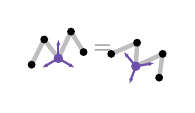
\begin{tikzpicture}[x=1mm, y=1mm, baseline={([yshift=-0.52em]current bounding box.north)}]
    \pictochain{0}
    \node[font=\footnotesize, text=ETHGray] at (9.0,0) {=};
    \begin{scope}[shift={(11.4,0.9)}, rotate=-40]
      \pictochain{-40}
    \end{scope}
\end{tikzpicture}}
\newcommand{\pictomirror}{
  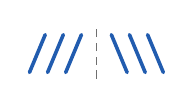
\begin{tikzpicture}[x=1mm, y=1mm, baseline={([yshift=-0.52em]current bounding box.north)}]
    \foreach \x in {0,2.3,4.6} \draw[ETHBlue, line width=1.3pt, line cap=round] (\x,-2.4) -- (\x+2,2.4);
    \draw[ETHGray, line width=0.5pt, densely dashed] (8.5,-3.2) -- (8.5,3.2);
    \foreach \x in {10.4,12.7,15} \draw[ETHBlue, line width=1.3pt, line cap=round] (\x+2,-2.4) -- (\x,2.4);
\end{tikzpicture}}

% The drawings of the backup slides. \pictoatoms: the backbone frame built from N, C-alpha, C.
% \pictomirrorpage: a residue and an atom above the page, and their mirror image.
\newcommand{\Tg}{T_{\text{global}}}
\newcommand{\pictoatoms}{
  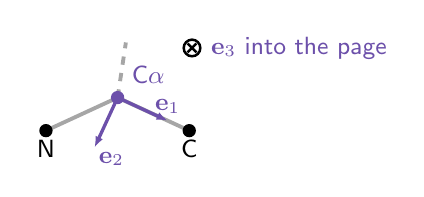
\begin{tikzpicture}[x=7mm, y=7mm]
    \coordinate (N) at (-1.3,-0.6); \coordinate (CA) at (0,0); \coordinate (C) at (1.3,-0.6);
    \draw[black!35, line width=1.4pt] (N) -- (CA) -- (C);
    \draw[black!35, line width=1.4pt, dashed] (CA) -- (0.15,1.0);
    \fill[black] (N) circle (2.4pt) node[below, font=\small] {N};
    \fill[black] (C) circle (2.4pt) node[below, font=\small] {C};
    \draw[CalloutPurple, line width=1.2pt, -{Latex[length=4pt]}] (CA) -- (-24.8:1.0) node[above, font=\small, text=CalloutPurple, inner sep=2pt] {$\mathbf e_1$};
    \draw[CalloutPurple, line width=1.2pt, -{Latex[length=4pt]}] (CA) -- (245.2:1.0) node[below right, font=\small, text=CalloutPurple, inner sep=1pt] {$\mathbf e_2$};
    \fill[CalloutPurple] (CA) circle (2.4pt);
    \node[font=\small, text=CalloutPurple, anchor=south west] at (0.08,0.08) {C$\alpha$};
    \draw[line width=0.9pt] (1.35,0.9) circle (3pt); \draw[line width=0.9pt] (1.35-0.08,0.9-0.08) -- (1.35+0.08,0.9+0.08) (1.35-0.08,0.9+0.08) -- (1.35+0.08,0.9-0.08);
    \node[font=\small, text=CalloutPurple, anchor=west] at (1.52,0.9) {$\mathbf e_3$ into the page};
\end{tikzpicture}}
\newcommand{\pictomirrorpage}{
  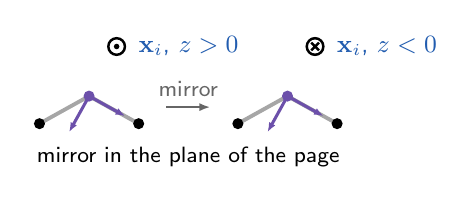
\begin{tikzpicture}[x=7mm, y=7mm]
    \foreach \dx/\lab in {0/{$z>0$}, 3.6/{$z<0$}} {
      \begin{scope}[shift={(\dx,0)}]
        \draw[black!35, line width=1.4pt] (-0.9,-0.5) -- (0,0) -- (0.9,-0.5);
        \fill[black] (-0.9,-0.5) circle (2pt); \fill[black] (0.9,-0.5) circle (2pt);
        \draw[CalloutPurple, line width=1.1pt, -{Latex[length=3.5pt]}] (0,0) -- (-29:0.75);
        \draw[CalloutPurple, line width=1.1pt, -{Latex[length=3.5pt]}] (0,0) -- (241:0.75);
        \fill[CalloutPurple] (0,0) circle (2pt);
        \draw[line width=0.9pt] (0.5,0.9) circle (3pt);
        \node[font=\small, anchor=west, text=ETHBlue] at (0.72,0.9) {$\mathbf x_i$, \lab};
      \end{scope}
    }
    \fill (0.5,0.9) circle (1pt);
    \draw[line width=0.9pt] (3.6+0.5-0.07,0.9-0.07) -- (3.6+0.5+0.07,0.9+0.07) (3.6+0.5-0.07,0.9+0.07) -- (3.6+0.5+0.07,0.9-0.07);
    \draw[black!60, line width=0.9pt, -{Latex[length=4pt]}] (1.4,-0.2) -- (2.2,-0.2) node[midway, above, font=\footnotesize] {mirror};
    \node[font=\footnotesize] at (1.8,-1.1) {mirror in the plane of the page};
\end{tikzpicture}}
% Intuition insets beside the architecture figures.
% \frameinset: all frames start at the origin, after the 8 layers each residue has its own frame.
\newcommand{\frameinset}{
  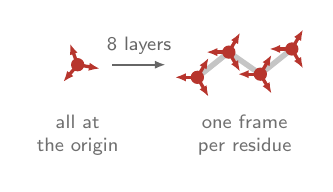
\begin{tikzpicture}[x=4mm, y=4mm]
    \frameaxes{(0,0)}{20}
    \node[font=\scriptsize, text=ETHGray, anchor=north, align=center] at (0,-1.3) {all at\\the origin};
    \draw[black!60, line width=0.8pt, -{Latex[length=4pt]}] (1.1,0) -- (2.8,0) node[midway, above, font=\scriptsize] {8 layers};
    \begin{scope}[shift={(3.8,-0.4)}]
      \draw[ETHGray!40, line width=2pt, line join=round, line cap=round] (0,0) -- (1.0,0.8) -- (2.0,0.1) -- (3.0,0.9);
      \foreach \p/\a in {(0,0)/10, (1.0,0.8)/-30, (2.0,0.1)/40, (3.0,0.9)/-10} {\frameaxes{\p}{\a}}
      \node[font=\scriptsize, text=ETHGray, anchor=north, align=center] at (1.5,-0.9) {one frame\\per residue};
    \end{scope}
\end{tikzpicture}}
% \rowinset: one MSA row, residue i attends to j, the pair cell ij is the bias.
\newcommand{\rowinset}{% the input sequence of the alignment slide, K at i = 3 attends to E at j = 9, biased by the pair cell (3,9)
  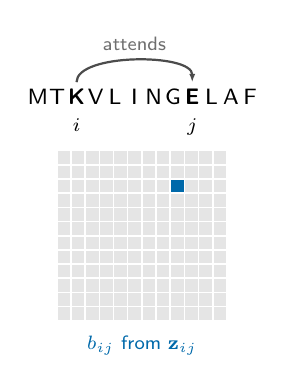
\begin{tikzpicture}[x=1mm, y=1mm]
    \foreach \aa [count=\c] in {M,T,K,V,L,I,N,G,E,L,A,F} \node[font=\footnotesize\sffamily, inner sep=0pt] at (\c*2.45,0) {\aa};
    \node[font=\footnotesize\sffamily\bfseries, inner sep=0pt, fill=white] at (3*2.45,0) {K};
    \node[font=\footnotesize\sffamily\bfseries, inner sep=0pt, fill=white] at (9*2.45,0) {E};
    \node[font=\scriptsize, anchor=north] at (3*2.45,-1.6) {$i$};
    \node[font=\scriptsize, anchor=north] at (9*2.45,-1.6) {$j$};
    \draw[black!70, line width=0.8pt, -{Latex[length=3pt]}] (3*2.45,1.8) .. controls (3*2.45,5.5) and (9*2.45,5.5) .. (9*2.45,1.8);
    \node[font=\scriptsize, text=ETHGray, anchor=south] at (6*2.45,4.6) {attends};
    \begin{scope}[shift={(2.45+2.5,-7)}]
      \foreach \r in {0,...,11} \foreach \c in {0,...,11} \fill[black!10] (\c*1.8,-\r*1.8) rectangle ++(1.6,-1.6);
      \fill[CalloutBlue] (8*1.8,-2*1.8) rectangle ++(1.6,-1.6);
      \node[font=\scriptsize, text=CalloutBlue, anchor=north] at (10.7,-22.2) {$b_{ij}$ from $\mathbf z_{ij}$};
    \end{scope}
\end{tikzpicture}}
% \fapeinset: atom i in frame k in both structures, the gap is d_ki (indices as in the paper's Fig. 3f).
\newcommand{\fapeinset}{
  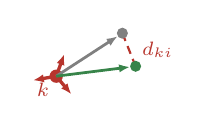
\begin{tikzpicture}[x=4.2mm, y=4.2mm]
    \frameaxes{(0,0)}{100}
    \draw[black!50, line width=1pt, -{Latex[length=4pt]}, shorten >=2pt] (0,0) -- (2.0,1.3);
    \draw[CalloutGreen, line width=1pt, -{Latex[length=4pt]}, shorten >=2pt] (0,0) -- (2.4,0.3);
    \draw[ETHRed, densely dashed, line width=0.8pt] (2.0,1.3) -- (2.4,0.3) node[midway, right=1pt, font=\scriptsize, text=ETHRed] {$d_{ki}$};
    \fill[black!50] (2.0,1.3) circle (2pt); \fill[CalloutGreen] (2.4,0.3) circle (2pt);
    \node[font=\scriptsize, text=framecol] at (-0.4,-0.4) {$k$};
\end{tikzpicture}}
% A signed number in the text font: -2.3 gets a real minus sign, 2.2 becomes +2.2
\newcommand{\signed}[1]{\expandafter\signedaux#1\relax}
\def\signedaux#1#2\relax{\ifx-#1\textminus#2\else+#1#2\fi}

% One outline slide after the title, not a repeat before every section
\AtBeginSection[]{}

% Metadata
% The line under the title names the paper. It is part of \title so that it stands above the presenters.
\title{Highly accurate protein structure\texorpdfstring{\\}{ }prediction with AlphaFold%
\texorpdfstring{\\[-0.5mm]{\usebeamerfont{date}Paper by Jumper et al., \textit{Nature} 596 (2021)}}{}}
\author{Evita Bosch Pokunevich \and Ben Bullinger}
\institute[ETH Z\"urich \\ Department of Computer Science]{ETH Z\"urich, Department of Computer Science}
\date[]{Machine Learning for Genomics (263-5351-00L), Fall 2026}

\begin{document}

% Working notes for us, taken during slide meetings. Set \worknotesfalse before the upload.
\newif\ifworknotes \worknotesfalse
\ifworknotes
{\setbeamertemplate{footline}{}
  \begin{frame}[t,noframenumbering]{Notes from Ben, not part of the talk}
    \begin{itemize}
      \item Side chain: now explained on slide 2 in one clause (Ben, 14 October). The whole deck was revised on 14 October along the four facts of slide 6, see \texttt{WORK-SPLIT.md}.
    \end{itemize}
\end{frame}}
\fi

{\setbeamertemplate{footline}{}
  \begin{frame}[noframenumbering]
    \vspace{12mm}
    {\fontsize{24}{28}\selectfont\bfseries Highly accurate protein structure\\prediction with AlphaFold\par}
    \vspace{4mm}
    {\large Jumper et al., \textit{Nature} 596 (2021) \ck{JEP+21}\par}
    \vspace{10mm}
    {Evita Bosch Pokunevich \quad Ben Bullinger\par}
    \vspace{2mm}
    {\scriptsize\href{https://github.com/BenBullinger/ML4Genomics-Presentation-AF2}{\color{ETHGray}\texttt{github.com/BenBullinger/ML4Genomics-Presentation-AF2}}\par}
    \vspace{3mm}
    {\color{ETHGray}Machine Learning for Genomics (263-5351-00L), ETH Z\"urich, Fall 2026\par}
\end{frame}}

% ---------------------------------------------------------------------------------------------
% Order of the talk: every term is defined on the slide where it first appears, nothing points
% forward. Problem, benchmark, pipeline, the four properties, the inputs, the Evoformer, the
% structure module, the loss, training, then results, limitations, what followed, summary.
% ---------------------------------------------------------------------------------------------
\section{The problem}

\begin{frame}[t]{Protein Structure Prediction}
  \begin{columns}[T,onlytextwidth]
    \begin{column}{0.5\textwidth}
      \vspace{3mm}
      {\LARGE SIFSYITESTGTPS\ldots\hfill
      \tikz[baseline=-0.6ex]\draw[line width=1.3pt, -{Latex[length=6pt]}] (0,0) -- (16mm,0);\hspace{2mm}\par}
      \vspace{1.5mm}
      {\small\color{ETHGray} Amino Acid Residues = Amino Acids after being incorporated into protein\par}
      \vspace{8mm}
      \key{The network predicts the 3D position of heavy atoms}
      \vspace{1mm}
      {\small\color{ETHGray} Heavy atoms = every atom except hydrogen\par}
    \end{column}
    \begin{column}{0.48\textwidth}
      \vspace{-8mm}
      \begin{marked}[0.95\linewidth]{1}{176 634 305 65}
        \fill[cover] (0.002,0.87) rectangle (0.07,1.01);
      \end{marked}\par
      \vspace{0.5mm}{\centering\small{\color{PaperGreen}Experiment} and {\color{PaperBlue}prediction}\par}
    \end{column}
  \end{columns}
  \reffootnote{\ck{JEP+21} Fig.~1b}
\end{frame}

% ---------------------------------------------------------------------------------------------
\section{The benchmark}

\begin{frame}[t]{The Benchmark: CASP14}
  \begin{columns}[T,onlytextwidth]
    \begin{column}{0.6\textwidth}
      \begin{marked}[0.7\linewidth]{1}{40 597 440 70}
      \end{marked}
    \end{column}%
    \hspace{-40mm}
    \begin{column}{0.5\textwidth}
      \vspace{6mm}
      \say{\textbf{CASP14}:  Critical Assessment of protein Structure Prediction
        \par\vspace{1.5mm}
        \say{\small\color{ETHGray} May-July 2020\par}
        \par\vspace{2mm}
        Blind test: experimental structures are not revealed until the end of experiment.
        \par\vspace{4mm}
        \r{A} (angstrom) = unit equal to $10^{-10}$ meters.
      }
      \key{Smaller RMSD means a closer structural match}
    \end{column}%
  \end{columns}
  \reffootnote{\ck{JEP+21}, Fig.~1a, The performance of AlphaFold on the CASP14 dataset (n = 87 protein domains) relative to the top-15 entries (out of 146 entries)}
\end{frame}

\begin{frame}[t]{Predicted Confidence}
  \begin{columns}[T,onlytextwidth]
    \begin{column}{0.6\textwidth}
      \vspace{6mm}
      \begin{marked}[\linewidth]{2}{40 483 302 180.5}
        \node[callout text, anchor=north west, align=left, text height=, text depth=] at (0.115,0.97) {confidence \\   vs\\  accuracy};
      \end{marked}
    \end{column}%
    \begin{column}{0.38\textwidth}
      \vspace{6mm}
      \say{\textit{(p)}LDDT: \textit{(Predicted)} Local Distance Difference test
        \vspace{3mm}
      {\par \color{ETHGray}Local accuracy score calculated per residue, averaged over protein; 0 to 100.}}
      \key{pLDDT is accurate as model's confidence score}
    \end{column}%
  \end{columns}
  \reffootnote{\ck{JEP+21}, Fig.~2c, Confidence score compared to the true accuracy on chains}
\end{frame}

% ---------------------------------------------------------------------------------------------
\section{The network}

% The frame of the talk. The paper (p. 584) describes the network as "based on the
% evolutionary, physical and geometric constraints of protein structures". Four such properties
% of the problem, known before training, and what the network builds in because of each. The
% design column uses no term that is defined later in the talk.
\begin{frame}[t]{Design Constraints}
  \props{1,2,3}\par
  \vspace{-1mm}
  % Every row is a band of the same height. Badge, pictogram and both text cells are centred
  % on the band's midline. The texts share one baseline, 1.1 mm below the midline, so that letters
  % with descenders do not shift a line. Nodes are set in the text font, since every node defaults to sans.
  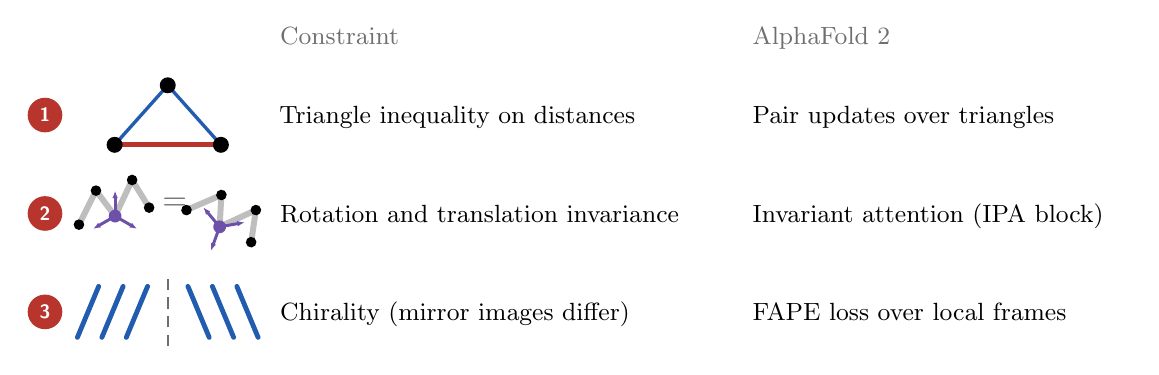
\begin{tikzpicture}[x=1mm, y=1mm, cell/.style={anchor=west, align=left, inner sep=0pt, font=\small, execute at begin node={\rmfamily\hyphenpenalty=10000}}]
    \node[cell, anchor=base west, text=ETHGray] at (32,-5.1) {Constraint};
    \node[cell, anchor=base west, text=ETHGray] at (92,-5.1) {AlphaFold 2};
    \foreach \n/\picto/\known/\built in {
      1/\pictotriangle/{Triangle inequality on distances}/{Pair updates over triangles},
      2/\pictorotate/{Rotation and translation invariance}/{Invariant attention (IPA block)},
    3/\pictomirror/{Chirality (mirror images differ)}/{FAPE loss over local frames}} {
      \coordinate (m) at (0,-1.5-\n*12.5);
      \fill[ETHRed] ($(m)+(2.2,0)$) circle (2.2mm);
      \node[font=\scriptsize\sffamily\bfseries, text=white, inner sep=0pt] at ($(m)+(2.2,0)$) {\n};
      \node[inner sep=0pt] at ($(m)+(17,0)$) {\scalebox{1.35}{\picto}};
      \node[cell, anchor=base west, text width=57mm] at ($(m)+(32,-1.1)$) {\known};
      \node[cell, anchor=base west, text width=48mm] at ($(m)+(92,-1.1)$) {\built};
    }
  \end{tikzpicture}
  \par\vspace{3mm}
\end{frame}

\begin{frame}[t]{Network Architecture}
  \vspace{-1mm}
  \begin{marked}[\linewidth]{1}{40 419 25 214}
    \fill[cover] (0.002,0.93) rectangle (0.04,1.01);
    % Red callouts name the parts the talk comes back to. The MSA is spelled out here.
    \callbox{fig1e/msa}
    \begin{scope}
      \draw[callout]
      ([shift={(-1mm,-0.5mm)}]\bx{fig1e/templates}{x0},\bx{fig1e/templates}{y0})
      rectangle
      ([shift={(1mm,9mm)}]\bx{fig1e/templates}{x1},\bx{fig1e/templates}{y1});
    \end{scope}   % the pairing icon sits 0.8 mm above the templates
    \callbox{fig1e/evoformer}
    \callbox{fig1e/structure}
    \callbox{fig1e/recycling}
    \boxlabel[align=center]{fig1e/msa}{above}{Multiple sequence\\alignment (MSA)}
    \boxlabel{fig1e/templates}{below}{Pair Features}
    \boxlabel{fig1e/evoformer}{above}{Evoformer}
    \boxlabel{fig1e/structure}{above}{Structure module}
    \boxlabel{fig1e/recycling}{below}{Recycled three times}
  \end{marked}
  \par\vspace{1mm}
  {\small\color{ETHGray} \textit{Recycling}: execute network multiple times on the same input.\par}
  \reffootnote{\ck{JEP+21}, Fig.~1e}
\end{frame}

% ---------------------------------------------------------------------------------------------
\subsection{The inputs}

\begin{frame}[t]{Multiple Sequence Alignment (MSA)}
  \begin{columns}[T,onlytextwidth]
    \begin{column}{0.6\textwidth}
      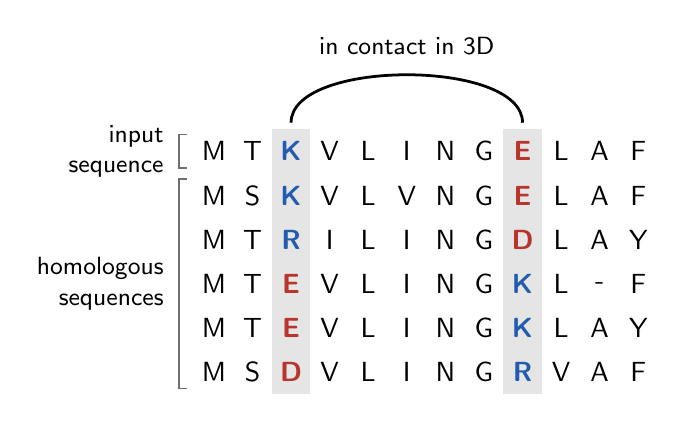
\begin{tikzpicture}[x=4.9mm, y=5.6mm]
        \fill[ETHGray!18] (2.5,-6.5) rectangle (3.5,-0.5);
        \fill[ETHGray!18] (8.5,-6.5) rectangle (9.5,-0.5);
        \foreach \row [count=\r] in \msarows {
          \foreach \aa [count=\c] in \row {
            \ifnum\c=3 \else\ifnum\c=9 \else
            \node[font=\sffamily, inner sep=0pt] at (\c,-\r) {\aa};
            \fi\fi
          }
        }
        % The two columns that change together: positive charge blue, negative charge red
        \foreach \a/\ca/\b/\cb [count=\r] in {K/ETHBlue/E/ETHRed, K/ETHBlue/E/ETHRed, R/ETHBlue/D/ETHRed,
        E/ETHRed/K/ETHBlue, E/ETHRed/K/ETHBlue, D/ETHRed/R/ETHBlue} {
          \node[font=\sffamily\bfseries, text=\ca, inner sep=0pt] at (3,-\r) {\a};
          \node[font=\sffamily\bfseries, text=\cb, inner sep=0pt] at (9,-\r) {\b};
        }
        \draw[line width=1pt] (3,-0.35) .. controls (3,1.1) and (9,1.1) .. (9,-0.35);
        \node[font=\small] at (6,1.4) {in contact in 3D};
        % brackets tie each label to its rows: row 1 the input, rows 2 to 6 its homologues
        \foreach \top/\bot in {-0.62/-1.38, -1.62/-6.38}
        \draw[ETHGray, line width=0.6pt] (0.3,\top) -- (0.1,\top) -- (0.1,\bot) -- (0.3,\bot);
        \node[font=\small, anchor=east, align=right] at (-0.05,-1) {input\\sequence};
        \node[font=\small, anchor=east, align=right] at (-0.05,-4) {homologous\\sequences};
      \end{tikzpicture}
    \end{column}
    \begin{column}{0.38\textwidth}
      \vspace{20.1mm}% centres the text on the six rows of the alignment
      \say{\textit{Co-evolution}: residues in contact change together across homologous proteins.

        {\small\color{ETHGray} Homologues = evolutionary related\par}
      }

    \end{column}
  \end{columns}
  \reffootnote{Illustration after \ck{MCS+11}}
\end{frame}

% Proposal (Ben) for the placeholder: the pair representation on its own, replacing the combined
% MSA and pair slide. Axes and asymmetry: SI 1.5, Algorithms 3 and 4, Fig. 3b. Templates: SI 1.2.9
% (template_distogram), Algorithm 2 line 13. Distance loss: SI 1.9.8.
\begin{frame}[t]{Pair Representation}
  \begin{columns}[T,onlytextwidth]
    \begin{column}{0.46\textwidth}
      \centering
      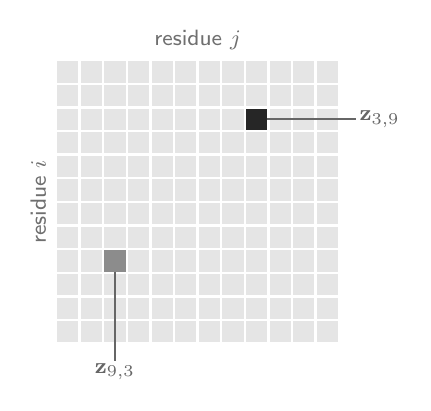
\begin{tikzpicture}[x=1mm, y=1mm, lab/.style={font=\footnotesize, inner sep=1pt}]
        \foreach \r in {0,...,11} \foreach \c in {0,...,11} \fill[black!10] (\c*3,-\r*3) rectangle ++(2.7,-2.7);
        \fill[black!85] (8*3,-2*3) rectangle ++(2.7,-2.7);
        \fill[black!45] (2*3,-8*3) rectangle ++(2.7,-2.7);
        \draw[black!60, line width=0.5pt] (8*3+2.7,-2*3-1.35) -- (38,-2*3-1.35) node[lab, anchor=west] {$\mathbf z_{3,9}$};
        \draw[black!60, line width=0.5pt] (2*3+1.35,-8*3-2.7) -- (2*3+1.35,-38) node[lab, anchor=north] {$\mathbf z_{9,3}$};
        \node[lab, text=ETHGray, anchor=south] at (17.85,1) {residue $j$};
        \node[lab, text=ETHGray, anchor=south, rotate=90] at (-1,-17.85) {residue $i$};
      \end{tikzpicture}
    \end{column}
    \begin{column}{0.52\textwidth}
      \vspace{3mm}
      \say{\textit{Pair representation} $\mathbf z_{ij}$: one vector per ordered pair of residues. $\mathbf z_{ij}$ and $\mathbf z_{ji}$ can differ.}
      \say{Start: the two amino acids, their offset $i - j$, and their distance in \textit{templates}, known structures of related proteins.}
    \end{column}
  \end{columns}
  \vspace{2mm}
  \key{An auxiliary loss trains $\mathbf z_{ij} + \mathbf z_{ji}$ to predict the distance of $i$ and $j$.}
  \reffootnote{\ck{JEP+21}, p.~585, Fig.~3b. SI 1.2.9, 1.5, Algorithms 2 to 4. Distance loss: SI 1.9.8}
\end{frame}

% ---------------------------------------------------------------------------------------------
\subsection{The Evoformer}

\begin{frame}[t]{The Evoformer Block}

  \begin{marked}[\linewidth]{3}{40 616 25 52}
    \fill[cover] (0.015,0.93) rectangle (0.04,1.01);
    % the paper's 48-blocks label, too small to read, re-set in the label font
    \fill[cover] (0.426,0.938) rectangle (0.562,0.998);
    \node[figure label, font=\scriptsize, fill=white, inner sep=1.5pt] at (0.494,0.968) {48 blocks, no shared weights};
    % from the pair line up into the row attention box
    \draw[callout, fill=none, line width=1.4pt, -{Latex[length=5pt]}] let \p1=(\bx{fig3a/rowatt}{x0},0.225), \p2=(\bx{fig3a/rowatt}{x1},0.225) in ($(\p1)!0.5!(\p2) + (0,0.012)$) -- ($(\p1)!0.5!(\p2) - (0,0.225) + (0,\bx{fig3a/rowatt}{y0}) - (0,\boxpad)$);
    \node[callout text, anchor=west, align=left] at (0.172,0.41) {pair to MSA:\\attention bias};
    \callbox{fig3a/opm}
    \draw[callout, fill=none, line width=1.4pt] let \p1=(\bx{fig3a/opm}{x0},0.735), \p2=(\bx{fig3a/opm}{x1},0.735) in ($(\p1)!0.5!(\p2)$) -- ($(\p1)!0.5!(\p2) - (0,0.735) + (0,\bx{fig3a/opm}{y1}) + (0,\boxpad)$);
    \draw[callout, fill=none, line width=1.4pt, -{Latex[length=5pt]}] let \p1=(\bx{fig3a/opm}{x0},\bx{fig3a/opm}{y0}), \p2=(\bx{fig3a/opm}{x1},\bx{fig3a/opm}{y0}) in ($(\p1)!0.5!(\p2) - (0,\boxpad)$) -- ($(\p1)!0.5!(\p2) - (0,\bx{fig3a/opm}{y0}) + (0,0.245)$);
    \node[callout text, anchor=west, align=left] at (0.43,0.545) {MSA to pair:\\outer product mean};
    \draw[callout, fill=none, rounded corners=0pt] (\bx{fig3a/triangles}{x0},-0.01) -- (\bx{fig3a/triangles}{x0},-0.05) -- (\bx{fig3a/triangles}{x1},-0.05) -- (\bx{fig3a/triangles}{x1},-0.01);
    \node[callout text, anchor=north] at (0.592,-0.06) {triangle layers};
    \node[figure label, font=\small, anchor=south west] at (0.028,0.84) {$\mathbf m_{si}$};
    \node[figure label, font=\small, anchor=north west] at (0.028,0.085) {$\mathbf z_{ij}$};
  \end{marked}
  \reffootnote{\ck{JEP+21}, Fig.~3a}
\end{frame}

\begin{frame}[t]{Evoformer: MSA Representation}{Self-attention for MSA representation}
  \par\vspace{-5mm}
  \begin{columns}[c,onlytextwidth]
    \begin{column}{0.76\textwidth}
      \begin{markedSI}[\linewidth]{1}{52bp 605bp 38bp 52bp}
        \callbox[cblue]{sfig2/pairbias}
        \boxlabel[cblue]{sfig2/pairbias}{below}{pair bias}
        \callcircle[cblue]{sfig2/plus}
      \end{markedSI}
    \end{column}
    \begin{column}{0.22\textwidth}
      \centering\rowinset
    \end{column}
  \end{columns}
  \vspace{1mm}
  \say{Residue $r_i$ attends to $r_j$ in its row, biased by the \bl{pair $b_{ij}$}.}
  \vspace{-1.5mm}
  {\par\centering $a_{sij} = \mathrm{softmax}_j\bigl(\tfrac{1}{\sqrt c}\,\mathbf q_{si}^{\top}\mathbf k_{sj} + \bl{b_{ij}}\bigr)$\par}
  \vspace{1mm}
  \reffootnote{\ck{JEP+21}, Suppl.\ Fig.~2, Algorithm 7}
\end{frame}

\begin{frame}[t]{Evoformer: Pair Representation}{1. Triangle inequality for the pair representation.}
  \props{1}\par\vspace{-6mm}
  \begin{center}
    \begin{marked}[0.83\linewidth]{3}{247 519.7 25 219}
      \node[figure label, font=\small\bfseries, anchor=base] at (0.23,1.165) {Multiplication};
      \node[figure label, text=ETHGray!90!black, anchor=base] at (0.115,1.008) {outgoing edge};
      \node[figure label, text=ETHGray!90!black, anchor=base] at (0.345,1.008) {incoming edge};
      \node[figure label, font=\small\bfseries, anchor=base] at (0.71,1.165) {Attention};
      \node[figure label, text=ETHGray!90!black, anchor=base] at (0.58,1.008) {around starting node};
      \node[figure label, text=ETHGray!90!black, anchor=base] at (0.84,1.008) {around ending node};
      % the two multiplicative updates, SI Algorithms 11 and 12
      \node[anchor=north, inner sep=1pt, font=\small] at (0.115,-0.04) {$\sum_k \mathbf a_{ik}\odot\mathbf b_{jk}$};
      \node[anchor=north, inner sep=1pt, font=\small] at (0.345,-0.04) {$\sum_k \mathbf a_{ki}\odot\mathbf b_{kj}$};
      \node[anchor=north, inner sep=1pt, font=\small, align=center] at (0.580,-0.04) {$ij$ from all $ik$\\bias $jk$};
      \node[anchor=north, inner sep=1pt, font=\small, align=center] at (0.830,-0.04) {$ij$ from all $kj$\\bias $ki$};
    \end{marked}
  \end{center}
  \vspace{-1.5mm}
  % graph view moved here from the Evoformer block (Fig. 3b: the cells ij drawn as directed edges i -> j)
  \begin{columns}[c,onlytextwidth]
    \begin{column}{0.62\textwidth}
      \say{\textit{Graph view}: residues are nodes, ordered pairs $ij$ are directed edges.}
      \say{\textit{Triangle inequality}: $d_{ij} \le d_{ik} + d_{kj}$ for every third residue $k$.}
    \end{column}
    \begin{column}{0.36\textwidth}
      \raggedleft\includegraphics[page=3,trim=55.8 532 424 204,clip,height=19mm]{literature/_AF2.pdf}
    \end{column}
  \end{columns}
  \reffootnote{\ck{JEP+21}, Fig.~3b and 3c, Supplementary Algorithms 11 to 14}
\end{frame}

% ---------------------------------------------------------------------------------------------
\subsection{The structure module}

% Proposal (Ben) for Evita's placeholder, from the figures she chose: what the frames and torsion
% angles of the structure module are of. SI 1.8.4: frames and torsion angles plus ideal bond
% lengths and angles fix every atom. Figures CC BY 4.0 [RKN+21] and CC BY 2.0 [HBP+10].
\begin{frame}[t]{Residue Geometry}
  \begin{columns}[b,onlytextwidth]
    \begin{column}{0.56\textwidth}
      \centering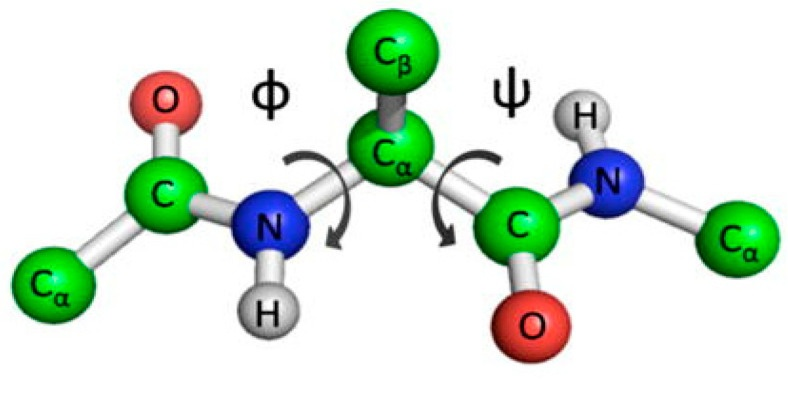
\includegraphics[width=0.95\linewidth]{literature/fig-backbone-phi-psi-RKN21.jpg}\par
      \vspace{1mm}
      {\small\color{ETHGray} Backbone torsion angles $\phi$, $\psi$\par}
    \end{column}
    \begin{column}{0.40\textwidth}
      \centering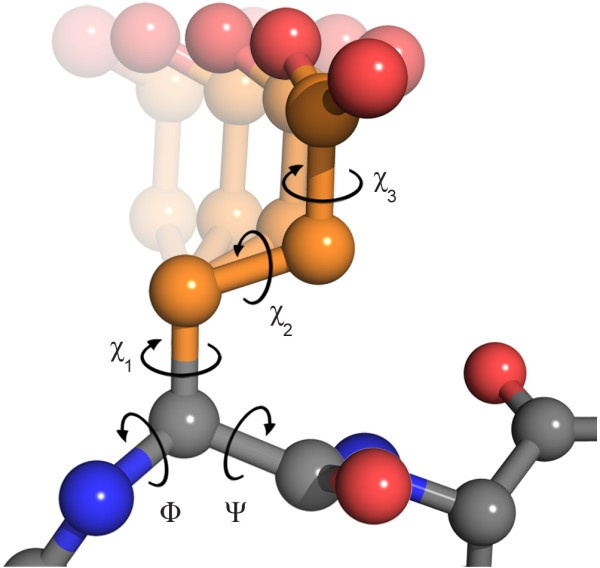
\includegraphics[height=34mm]{literature/fig-glutamate-chi-HBP10.jpg}\par
      \vspace{1mm}
      {\small\color{ETHGray} Side-chain torsion angles $\chi_1$ to $\chi_3$\par}
    \end{column}
  \end{columns}
  \vspace{2mm}
  \say{\textit{Backbone}: N, C$\alpha$, C along the chain. \textit{Side chain}: on C$\alpha$, 0 to 4 angles $\chi$.}
  \key{A frame per residue and its torsion angles fix every atom.}
  \reffootnote{Figures from \ck{RKN+21}, Fig.~3a, CC BY 4.0, and \ck{HBP+10}, Fig.~1, CC BY 2.0. \ck{JEP+21}, SI 1.8.4}
\end{frame}

% The structure module at the level of the supplement: Fig. 3d with the line numbers of
% Algorithm 20. The frame is defined here. The loss comes on the slide after IPA.
\begin{frame}[t]{The Structure Module}{2. Rotation and translation invariance.}
  \props{2}\par\vspace{-5mm}
  \begin{columns}[T,onlytextwidth]
    \begin{column}{0.6\textwidth}
      \begin{marked}[\linewidth]{3}{40 358 302 295}
        \setlength{\boxpad}{0.7mm}
        \fill[cover] (0.03,0.64) rectangle (0.07,0.73);
        \callbox{fig3d/ipa}
        \boxlabel{fig3d/ipa}{below}{IPA}
        \callbox[cpurple]{fig3d/update}
        \begin{scope}\setlength{\boxpad}{0.3mm}\callbox[cpurple]{fig3d/frames}
        \end{scope}   % the paper's label sits 0.7 mm under the frames
        \callbox[cgreen]{fig3d/atoms}
      \end{marked}
    \end{column}
    \begin{column}{0.38\textwidth}
      \say{In each of 8 layers \rd{\textit{invariant point attention} (IPA)} updates the input residue features and \pu{position and orientation of each frame}. Then, from frames and torsion angles $\chi$, \gn{all atom coordinates are computed}.}
      {\centering\colorlet{framecol}{CalloutPurple}\frameinset\par}
    \end{column}
  \end{columns}
  \vspace{1mm}
  \reffootnote{\ck{JEP+21}, Fig.~3d}
\end{frame}

% IPA at the level of the supplement: Suppl. Fig. 8 with the line numbers of Algorithm 22.
\begin{frame}[t]{Structure Module: Invariant Point Attention}{2. Rotation and translation invariance.}
  \props{2}\par\vspace{-5mm}
  \begin{columns}[T,onlytextwidth]
    \begin{column}{0.6\textwidth}
      \begin{markedSI}[\linewidth]{2}{55bp 501bp 55bp 55bp}
        \setlength{\boxpad}{0.7mm}
        \callbox[cblue]{sfig8/pairbias}
        \callbox{sfig8/dot}
        \callbox[cgreen]{sfig8/sqdist}
        \callcircle{sfig8/plus}
      \end{markedSI}
    \end{column}
    \begin{column}{0.38\textwidth}
      \vspace{1mm}
      \say{Logit: \rd{dot product}, plus \bl{pair bias}, minus the \gn{squared distances of the points}.}
      % the inset with a legend: frames, the 4 points of each residue, the distance for each p, the chain
      {\raggedright\colorlet{ipadist}{CalloutGreen}\colorlet{framecol}{CalloutPurple}\colorlet{ipaq}{black!70}
        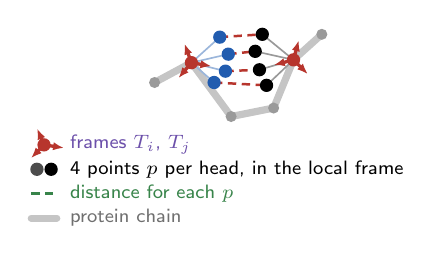
\begin{tikzpicture}[x=3.6mm, y=3.6mm, lab/.style={font=\scriptsize, inner sep=1pt, anchor=west}]
          \begin{scope}[shift={(4,0)}]\ipapair
          \end{scope}   % the drawing centred over the column, the legend stays flush left
          \begin{scope}[shift={(-1.2,-2.9)}, y=3.1mm]
            \frameaxes{(0,0)}{20}
            \node[lab, text=CalloutPurple] at (0.8,0) {frames $T_i$, $T_j$};
            \fill[black!70] (-0.25,-1.0) circle (2.4pt); \fill[black] (0.25,-1.0) circle (2.4pt);
            \node[lab] at (0.8,-1.0) {4 points $p$ per head, in the local frame};
            \draw[CalloutGreen, line width=0.9pt, densely dashed] (-0.45,-2.0) -- (0.45,-2.0);
            \node[lab, text=CalloutGreen] at (0.8,-2.0) {distance for each $p$};
            \draw[ETHGray!40, line width=2.6pt, line cap=round] (-0.45,-3.0) -- (0.45,-3.0);
            \node[lab, text=ETHGray] at (0.8,-3.0) {protein chain};
          \end{scope}
      \end{tikzpicture}\par}
    \end{column}
  \end{columns}
  {\par\centering $\rd{\mathbf q_i^{\top}\mathbf k_j} + \bl{b_{ij}} - \gn{\gamma\textstyle\sum_p \|T_i\circ\vec{\mathbf q}_{ip} - T_j\circ\vec{\mathbf k}_{jp}\|^2}$\par}
  \vspace{1.5mm}
  \key{A global rotation or translation leaves every weight unchanged.}
  \reffootnote{\ck{JEP+21}, p.~587. SI 1.8.2, Suppl.\ Fig.~8, Algorithm 22, one of 12 heads, constant weights omitted. Invariance proof on backup slide I}
\end{frame}

% FAPE at the level of the supplement: the paper's Fig. 3f and Algorithm 28. The total loss
% with the other heads follows on the training slide, where those heads are introduced.
\begin{frame}[t]{Loss: Frame Aligned Point Error}{3. Chirality (mirror images differ).}
  \props{3}\par\vspace{-5mm}
  \begin{columns}[T,onlytextwidth]
    \begin{column}{0.36\textwidth}
      \begin{marked}[\linewidth]{3}{468 380 22 332}
        \fill[cover] (0,0.8) rectangle (0.3,1.02);
      \end{marked}
    \end{column}
    \begin{column}{0.6\textwidth}
      \vspace{2mm}
      \say{\textit{Frame aligned point error} (FAPE): distance $\rd{d_{ki}}$ between atom $i$ in frame $k$, \gn{predicted} and {\color{ETHGray}true}.}
      {\par\centering $\mathcal L_{\text{FAPE}} = \tfrac{1}{10\,\text{\AA}}\,\mathrm{mean}_{k,i}\,\min(10\,\text{\AA}, \rd{d_{ki}})$\par}
      \vspace{2mm}
      {\centering\colorlet{framecol}{CalloutPurple}\scalebox{1.6}{\fapeinset}\par}
    \end{column}
  \end{columns}
  \vspace{2mm}
  \key{FAPE is invariant to rotations and translations. It distinguishes mirror images.}
  \reffootnote{\ck{JEP+21}, p.~587 and Fig.~3f. SI 1.9.2, Algorithm 28. Mirror argument on backup slide II}
\end{frame}

% ---------------------------------------------------------------------------------------------
\section{Training}

\begin{frame}[t]{Training Data and Loss}
  \vspace{-3mm}
  \begin{columns}[T,totalwidth=\textwidth]
    \begin{column}{0.55\textwidth}
      \say{\textit{Self-distillation}: training on predicted structures for 350,000 sequences without a known structure.}
      \vspace{0.5mm}
      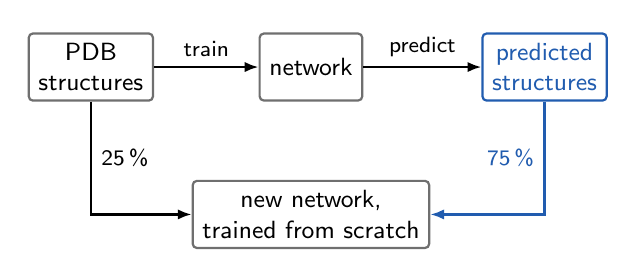
\begin{tikzpicture}[x=8.6mm, y=7.2mm,
          box/.style={draw=ETHGray, line width=0.8pt, rounded corners=1.5pt, font=\small, align=center,
          inner sep=3.5pt, minimum height=8.5mm},
        flow/.style={line width=0.9pt, -{Latex[length=5pt]}}]
        \node[box] (pdb) at (0,2.6) {PDB\\structures};
        \node[box] (net) at (3.25,2.6) {network};
        \node[box, draw=ETHBlue, text=ETHBlue] (pred) at (6.7,2.6) {predicted\\structures};
        \node[box] (new) at (3.25,0) {new network,\\trained from scratch};
        \draw[flow] (pdb) -- node[above, font=\footnotesize] {train} (net);
        \draw[flow] (net) -- node[above, font=\footnotesize] {predict} (pred);
        \draw[flow] (pdb) |- node[pos=0.25, right, font=\footnotesize] {25\,\%} (new);
        \draw[flow, ETHBlue] (pred) |- node[pos=0.25, left, font=\footnotesize] {75\,\%} (new);
      \end{tikzpicture}
    \end{column}
    \begin{column}{0.37\textwidth}
      \say{\textit{Masked MSA loss}: 15\,\% of entries hidden and predicted, as in BERT.}
      \vspace{0.5mm}
      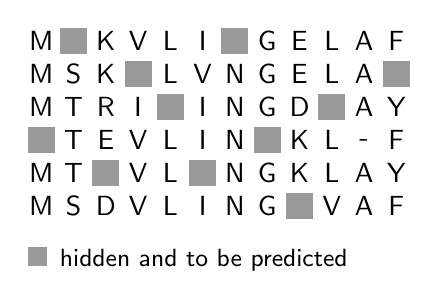
\begin{tikzpicture}[x=4.1mm, y=4.2mm]
        \foreach \row [count=\r] in \msarows {
          \foreach \aa [count=\c] in \row {
            \node[font=\sffamily, inner sep=0pt] at (\c,-\r) {\aa};
          }
        }
        \foreach \c/\r in {2/1, 7/1, 4/2, 12/2, 10/3, 5/3, 1/4, 8/4, 6/5, 3/5, 9/6}
        \fill[ETHGray!70] (\c-0.42,-\r-0.40) rectangle (\c+0.42,-\r+0.40);
        \node[font=\small, anchor=west, inner sep=0pt] at (0.58,-7.6) {\textcolor{ETHGray!70}{\rule{2.4mm}{2.4mm}}\enspace hidden and to be predicted};
      \end{tikzpicture}
    \end{column}
  \end{columns}
  \vspace{6mm}% the total loss belongs to the whole slide, not to one column
  \say{Total loss: FAPE (final and per layer), distances, masked MSA, pLDDT.}
  \key{Self-distillation considerably improves the accuracy.}
  \reffootnote{\ck{JEP+21}, p.~587. SI 1.3, 1.9, eq.~7, fine-tuning adds two terms. Self-distillation after \ck{XLHL20}, masking after \ck{DCLT19}}
\end{frame}

% ---------------------------------------------------------------------------------------------
\section{What makes it work}

\begin{frame}[t]{Ablation Study}
  \definebox{sfig9/mirrorhigh}{0.790}{0.766}{0.886}{0.912}   % the high cluster of the mirror column, set by hand
  \props{1,2,3}\par\vspace{-8.5mm}
  % GDT is used by both figures, so it is defined once above them, across the full width
  {\footnotesize\color{ETHGray} \textit{Global distance test} (GDT): mean percent of C$\alpha$ atoms within 1, 2, 4 and 8\,\AA\ of the experiment\par}
  \vspace{1.5mm}
  \begin{columns}[T,onlytextwidth]
    \begin{column}{0.6\textwidth}
      % Fig. 4a of the paper. The paper's 6 pt row labels, axis numbers and headers are covered
      % and re-set in the slide font; bars and error bars are the paper's.
      {\footnotesize\color{ETHGray} Accuracy change against the baseline\par}
      \raggedleft
      \begin{marked}[0.555\linewidth]{4}{310 556 28 46}
        \fill[cover] (-0.01,-0.01) rectangle (0.345,1.01);
        \fill[cover] (0.345,0.925) rectangle (1.01,1.01);
        \fill[cover] (0.345,-0.01) rectangle (1.01,0.09);
        \foreach \y/\lab/\ink in {
          0.882/{Self-distillation added}/ETHGray, 0.807/{Baseline}/black, 0.734/{No templates}/ETHGray,
          0.659/{No distogram head}/ETHGray, 0.583/{No raw MSA, statistics only}/ETHGray,
          0.505/{{\color{ETHRed}\bfseries 2}\enspace No IPA}/black, 0.437/{No masked-MSA head}/ETHGray,
          0.363/{No recycling}/ETHGray, 0.286/{{\color{ETHRed}\bfseries 1}\enspace No triangles, bias, gating}/black,
        0.213/{No end-to-end gradients}/ETHGray, 0.135/{No IPA and no recycling}/ETHGray}
        \node[font=\scriptsize, anchor=east, inner sep=1pt, text=\ink, text height=1.5ex, text depth=0.4ex] at (0.338,\y) {\lab};
        \foreach \x/\n in {0.376/\textminus20, 0.485/\textminus10, 0.598/0, 0.679/\textminus4, 0.769/\textminus2, 0.861/0, 0.950/2}
        \node[font=\scriptsize, anchor=north, inner sep=1pt] at (\x,0.095) {\n};
        \node[font=\scriptsize, anchor=south] at (0.49,0.93) {GDT};
        \node[font=\scriptsize, anchor=south] at (0.815,0.93) {lDDT-C$\alpha$};
      \end{marked}
    \end{column}
    \begin{column}{0.38\textwidth}
      {\scriptsize\color{ETHGray} Without FAPE: GDT against truth and mirror\par}
      \centering
      \begin{markedSI}[0.42\linewidth]{3}{158 547 290 45}
        % the paper's rotated column labels are covered below the plot area and the bottom
        % border is redrawn; the crop keeps the "0" tick label whole
        \fill[cover] (0.25,-0.03) rectangle (1.01,0.038);   % starts right of the 0 tick label
        \draw[black!25, line width=0.3pt] (0.165,0.032) -- (0.995,0.032);
        \node[font=\scriptsize, anchor=north] at (0.42,-0.01) {truth};
        \node[font=\scriptsize, anchor=north] at (0.83,-0.01) {mirror};
        % the supplement's y label ``Value'' re-set as GDT
        \fill[cover] (-0.01,0.25) rectangle (0.115,0.8);
        \node[font=\scriptsize, rotate=90, anchor=south] at (0.105,0.52) {GDT};
        \callbox{sfig9/lowgroup}
        \callbox{sfig9/mirrorhigh}
      \end{markedSI}
    \end{column}
  \end{columns}
  \say{{\color{ETHRed}\bfseries 3}\enspace Without FAPE, the model frequently predicts mirror images (SI 1.9.3).\\
  \rd{Red boxes}: low GDT against the truth, high GDT against the mirror.}
  \key{Triangle updates matter more than IPA. FAPE ensures the correct chirality.}
  \reffootnote{\ck{JEP+21}, Fig.~4a and Suppl.\ Fig.~9, labels re-set. GDT (Zemla 2003) on 87 CASP14 domains, lDDT-C$\alpha$ on PDB chains. SI 1.9.3}
\end{frame}

\begin{frame}[t]{Intermediate Structures}
  % Left: Fig. 4b of the paper. Right: the part of Fig. 1e from slide 5 that the plot's
  % axis comes from, with the same red frames. Its boxes are defined here, as fractions of
  % this narrower crop, so boxes.tex is unchanged.
  \definebox{fig1e-recap/evoformer}{0.2286}{0.2564}{0.3640}{0.9652}
  \definebox{fig1e-recap/structure}{0.6335}{0.2564}{0.7689}{0.9652}
  \definebox{fig1e-recap/recycling}{0.0239}{0.0033}{0.9456}{0.0910}
  \vspace{-1mm}
  \begin{columns}[T,onlytextwidth]
    \begin{column}{0.65\textwidth}
      \begin{marked}[\linewidth]{4}{309 415 25 272}
        \fill[cover] (0.002,0.9) rectangle (0.05,1.01);
        \fill[cover] (0.78,0.235) rectangle (0.965,0.44);
        \fill[cover] (0.005,0.42) rectangle (0.05,0.75);
        % the paper's axis numbers and axis title, replaced by larger ones
        \fill[cover] (0.052,0.16) rectangle (0.098,1.0);
        \fill[cover] (0.09,0.002) rectangle (0.975,0.178);
        \foreach \x/\n in {0.114/0, 0.3215/48, 0.5285/96, 0.7365/144, 0.9435/192}
        \node[font=\scriptsize, inner sep=1pt, anchor=north] at (\x,0.175) {\n};
        \foreach \y/\n in {0.2085/0, 0.3575/20, 0.5065/40, 0.6555/60, 0.8045/80, 0.9535/100}
        \node[font=\scriptsize, inner sep=1pt, anchor=east] at (0.098,\y) {\n};
        \foreach \x in {0.3215,0.5285,0.7365}
        \draw[ETHGray, line width=0.6pt, densely dashed] (\x,0.2085) -- (\x,0.965);
        \foreach \x/\n in {0.218/1, 0.425/2, 0.6325/3, 0.84/4}
        \node[figure label, font=\scriptsize, text=ETHGray] at (\x,0.275) {pass \n};
        \node[figure label, font=\scriptsize] at (0.525,0.075) {Evoformer block};
        \fill[cover] (0.005,0.45) rectangle (0.04,0.72);
        \node[figure label, font=\scriptsize, rotate=90, anchor=south] at (0.03,0.58) {GDT};
        % legend of the three curves, in one row above the plot
        \foreach \x/\c/\n in {0.2/PaperCurveBlue/{LmrP, domain 1}, 0.515/PaperCurveOrange/{LmrP, domain 2}, 0.83/PaperCurveGreen/{ORF8}} {
          \draw[\c, line width=1.2pt] (\x,1.045) -- ({\x+0.045},1.045);
          \node[font=\scriptsize, anchor=west, inner sep=1pt] at ({\x+0.05},1.045) {\n};
        }
      \end{marked}
    \end{column}
    \begin{column}{0.31\textwidth}
      \vspace{3mm}
      {\scriptsize\color{ETHGray} From slide 5\par}
      \vspace{0.5mm}
      \begin{marked}[\linewidth]{1}{258.8 419 41.4 214}
        \setlength{\boxpad}{0.5mm}
        \callbox{fig1e-recap/evoformer}
        \callbox{fig1e-recap/structure}
        \callbox{fig1e-recap/recycling}
        \boxlabel[font=\scriptsize, align=center, text height=, text depth=, xshift=-1.5mm]{fig1e-recap/evoformer}{above}{Evoformer,\\48 blocks}
        \boxlabel[font=\scriptsize, align=center, text height=, text depth=]{fig1e-recap/structure}{above}{One structure\\module per block}
        \boxlabel[font=\scriptsize]{fig1e-recap/recycling}{below}{Recycled three times: 4 passes}
      \end{marked}
    \end{column}
  \end{columns}
  \vspace{2mm}
  \say{\textit{Probing}: each of the 48 Evoformer blocks gets its own copy of the structure module, trained to predict the structure from that block's output. The main network is frozen.}
  \key{LmrP reaches its final structure early. ORF8 needs nearly the full depth.}
  \reffootnote{\ck{JEP+21}, p.~587, Fig.~4b and Fig.~1e, labels re-set, SI 1.14. LmrP: CASP14 target T1024. ORF8: T1064, SARS-CoV-2}
\end{frame}

\begin{frame}[t]{Limitations}
  \begin{columns}[T,onlytextwidth]
    \begin{column}{0.44\textwidth}
      \begin{marked}[\linewidth]{5}{64 585 352 61}
        \fill[cover] (0.59,0.185) rectangle (0.90,0.31);
        \fill[cover] (0.002,0.47) rectangle (0.049,0.66);
        % the paper's axis numbers and axis title, replaced by larger ones
        \fill[cover] (0.05,0.12) rectangle (0.108,1.0);
        \fill[cover] (0.11,0.002) rectangle (0.95,0.136);
        \foreach \k in {0,1,2,3,4}
        \node[font=\scriptsize, inner sep=1pt, anchor=north] at (0.1427+0.1876*\k,0.135) {10\textsuperscript{\k}};
        \foreach \y/\n in {0.1635/0, 0.3248/20, 0.4861/40, 0.6474/60, 0.8087/80, 0.97/100}
        \node[font=\scriptsize, inner sep=1pt, anchor=east] at (0.108,\y) {\n};
        \draw[ETHRed, line width=1.2pt, densely dashed] (0.4198,0.1635) -- (0.4198,0.985);
        \node[callout text, anchor=south] at (0.4198,0.99) {30};
        % limitation 1 of the text: the region below 30 effective sequences, where the curves drop
        \draw[callout] (0.148,0.53) rectangle (0.41,0.905);
        \node[inner sep=1.5pt, anchor=south west, text=ETHRed, font=\small\bfseries, execute at begin node=\rmfamily] at (0.148,0.905) {1};
        \node[figure label] at (0.52,0.035) {effective sequences in the MSA ($N_{\mathrm{eff}}$)};
        \node[figure label, anchor=south] at (0.108,1.01) {lDDT-C$\alpha$};
        \fill[white, opacity=0.85] (0.44,0.19) rectangle (0.97,0.46);
        \node[figure label, anchor=west] at (0.46,0.41) {template covers};
        \draw[PaperCurveOrange, line width=1.4pt] (0.475,0.325) -- (0.55,0.325);
        \node[figure label, anchor=west] at (0.57,0.325) {> 60\,\% of chain};
        \draw[PaperCurveBlue, line width=1.4pt] (0.475,0.24) -- (0.55,0.24);
        \node[figure label, anchor=west] at (0.57,0.24) {< 30\,\% of chain};
      \end{marked}
    \end{column}
    \begin{column}{0.55\textwidth}
      \vspace{8mm}
      % same numbers and headings as the exam slide, which answers with these two limitations
      {\color{ETHRed}\bfseries 1}\enspace\textbf{Proteins with few known relatives}\par
      \vspace{0.8mm}
      {\raggedright Accuracy drops below about 30 sequences.\\ {\color{PaperCurveOrange}With a template}, the drop is much smaller.\par}
      \vspace{4mm}
      {\color{ETHRed}\bfseries 2}\enspace
      \begin{tabular}[t]{@{}l@{}}\textbf{Domains whose shape}\\\textbf{comes from a complex}
      \end{tabular}\par
      \vspace{0.8mm}
      {\raggedright Much weaker if most contacts are inter-chain.\\ AlphaFold 2 takes one chain as input.\par}
    \end{column}
  \end{columns}
  \reffootnote{\ck{JEP+21}, p.~588, Fig.~5a, labels re-set. Recent PDB chains with at most 25\,\% of contacts to other chains. $N_{\mathrm{eff}}$: sequences after merging near-duplicates}
\end{frame}

% ---------------------------------------------------------------------------------------------
\section{Conclusion}

\begin{frame}[t]{Since AlphaFold 2}
  % The rows are sentences, so they are set in the text font. The source of each row stands
  % at its right end: first author, venue, year. Full references follow on the closing slides.
  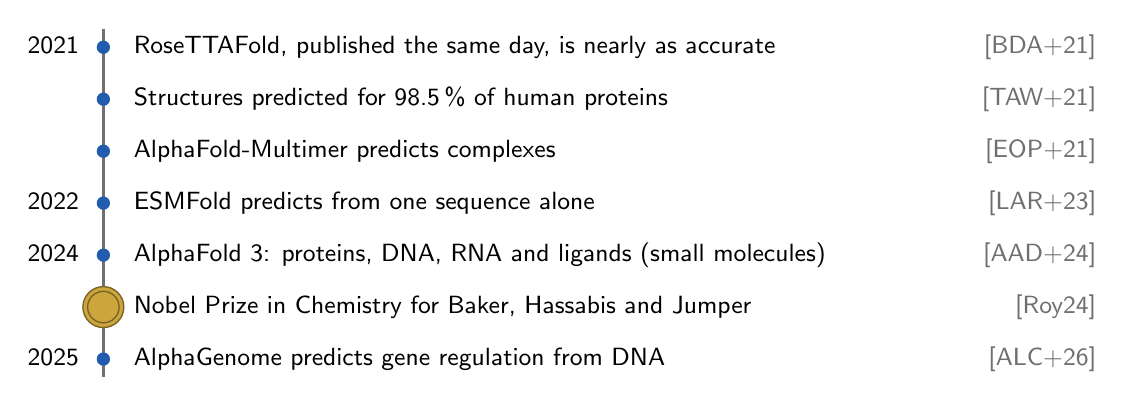
\begin{tikzpicture}[x=7.6mm, y=6.6mm]
    \draw[ETHGray, line width=1pt] (0,0.35) -- (0,-6.35);
    \foreach \y/\text/\cite in {
      0/{RoseTTAFold, published the same day, is nearly as accurate}/{\ck{BDA+21}},
      -1/{Structures predicted for 98.5\,\% of human proteins}/{\ck{TAW+21}},
      -2/{AlphaFold-Multimer predicts complexes}/{\ck{EOP+21}},
      -3/{ESMFold predicts from one sequence alone}/{\ck{LAR+23}},
      -4/{AlphaFold~3: proteins, DNA, RNA and ligands (small molecules)}/{\ck{AAD+24}},
      -5/{Nobel Prize in Chemistry for Baker, Hassabis and Jumper}/{\ck{Roy24}},
    -6/{AlphaGenome predicts gene regulation from DNA}/{\ck{ALC+26}}} {
      \fill[ETHBlue] (0,\y) circle (2.4pt);
      \node[anchor=mid west, inner sep=0pt, font=\rmfamily\small] at (0.5,\y) {\text};
      \node[anchor=mid east, inner sep=0pt, font=\rmfamily\small, text=ETHGray] at (16.6,\y) {\cite};
    }
    \foreach \y/\year in {0/2021, -3/2022, -4/2024, -6/2025}
    \node[anchor=mid east, inner sep=0pt, font=\rmfamily\small] at (-0.4,\y) {\year};
    % the Nobel row gets a medal in place of its dot: a gold disc on a short ribbon
    \fill[ETHBlue] (-0.12,-4.72) -- (0.12,-4.72) -- (0.06,-4.95) -- (-0.06,-4.95) -- cycle;
    \fill[Gold] (0,-5) circle (2.6mm);
    \draw[Gold!60!black, line width=0.5pt] (0,-5) circle (2.6mm);
    \draw[Gold!60!black, line width=0.5pt] (0,-5) circle (2.0mm);
  \end{tikzpicture}
  \par\vspace{2mm}
  \reffootnote{Full references at the end}
\end{frame}

% The follow-up paper's own verdict on each of the four design choices.
\begin{frame}[t]{Design Constraints in AlphaFold 3}
  \props{1,2,3}\par
  \vspace{-6mm}
  \begin{center}
    \begin{markedAFthree}[0.9\linewidth]{1}{44 344 30 329}
      \setlength{\boxpad}{0.7mm}
      \fill[cover] (0,0.88) rectangle (0.025,1.01);
      % red frames numbered with the constraints of slide 4, as on the ablation slide
      % the output structure, where the loss acts and where chirality is right or wrong; defined
      % here, measured on the slide render, so boxes.tex is unchanged
      \definebox{af3/output}{0.908}{0.21}{0.978}{0.475}
      \callbox{af3/pairformer}
      \callbox{af3/diffusion}
      \callbox{af3/output}
      \node[inner sep=1.5pt, anchor=south west, text=ETHRed, font=\small\bfseries, execute at begin node=\rmfamily] at ([xshift=1mm]\bx{af3/output}{x1},\bx{af3/output}{y0}) {3};
      \node[inner sep=1.5pt, anchor=north west, text=ETHRed, font=\small\bfseries, execute at begin node=\rmfamily] at (\bx{af3/pairformer}{x0},\bx{af3/pairformer}{y1}) {1};
      \node[inner sep=1.5pt, anchor=north east, text=ETHRed, font=\small\bfseries, execute at begin node=\rmfamily] at ([xshift=-1mm]\bx{af3/diffusion}{x0},\bx{af3/diffusion}{y1}) {2};
    \end{markedAFthree}
  \end{center}
  \vspace{1mm}
  \say{{\color{ETHRed}\bfseries 1}\enspace The Pairformer keeps the triangle updates.}
  \say{{\color{ETHRed}\bfseries 2}\enspace A diffusion module outputs atom coordinates, without \pu{frames} or IPA.}
  \say{{\color{ETHRed}\bfseries 3}\enspace
    \begin{tabular}[t]{@{}l@{}}An aligned mean squared error replaces FAPE.\\Chirality is wrong in 4.4\,\% of ligand predictions.
  \end{tabular}}
  \reffootnote{\ck{AAD+24}, Fig.~1d, p.~494 to 497, Suppl.\ 3.7.1. 4.4\,\%: chirality violation rate on the PoseBusters benchmark, after a ranking penalty}
\end{frame}

\begin{frame}[t]{Summary}
  \props{1,2,3}
  % Fig. 1e of slide 5 with the three constraints placed: 1 in the Evoformer, 2 in the structure
  % module, 3 on the output structure, as on the AlphaFold 3 slide
  \vspace{-8mm}
  \begin{center}
    \begin{marked}[0.55\linewidth]{1}{40 419 25 214}
      \fill[cover] (0.002,0.93) rectangle (0.04,1.01);
      \callbox{fig1e/evoformer}
      \callbox{fig1e/structure}
      \callbox{fig1e/output}
      \boxlabel[font=\small\bfseries, execute at begin node=\rmfamily]{fig1e/evoformer}{above}{1}
      \boxlabel[font=\small\bfseries, execute at begin node=\rmfamily]{fig1e/structure}{above}{2}
      \boxlabel[font=\small\bfseries, execute at begin node=\rmfamily]{fig1e/output}{right}{3}
    \end{marked}
  \end{center}
  \vspace{-1mm}
  % GDT changes: Fig. 4a, mean of the three seeds, read off against the paper's tick marks
  {\small\setlength{\tabcolsep}{1.4mm}
    \begin{tabular}{@{}llrl@{}}
      & & {\color{ETHGray} Removal in AlphaFold 2} & {\color{ETHGray} AlphaFold 3} \\[0.5mm]
      {\color{ETHRed}\bfseries 1} & triangle updates on the pairs & \textminus4.6 GDT & kept \\
      {\color{ETHRed}\bfseries 2} & IPA in the structure module & \textminus2.3 GDT & dropped \\
      {\color{ETHRed}\bfseries 3} & FAPE in local frames & mirror images & dropped, 4.4\,\% wrong chirality \\
  \end{tabular}\par}
  \vspace{1mm}
  \key{AlphaFold 2 reaches atomic accuracy in CASP14.\\ Triangle updates, IPA and FAPE let it learn efficiently from limited data.}
  \vspace{1mm}{\small\color{ETHGray} AlphaFold 3 also predicts DNA, RNA and ligands, for which AlphaFold 2 defines no frames.\\ Rotations are learned from randomly rotated training data instead.\par}
  \reffootnote{\ck{JEP+21}, p.~584 and 588, Fig.~4a, mean of three seeds. \ck{AAD+24}, p.~494 to 497. Figures reproduced under CC BY 4.0}
\end{frame}

% ---------------------------------------------------------------------------------------------
% Part 2 of the guidelines (10 minutes): the exam question after the conclusion, then at least
% two questions for the audience and a moderated discussion.
\section{Questions}

% The question from Lovro Rabuzin, for presentation 5. The two cases are the two limits
% the paper names on p. 588. Fig. 5a is already on the limitations slide. Fig. 5b is three
% copies of one protein, the case that still works.
\begin{frame}[t]{Exam Question}
  % Both answers are the two limitations the paper names, p. 588 ("MSA depth and cross-chain
  % contacts"); depth as defined in the Fig. 5 caption and Methods p. 591 (Neff, 80 % identity).
  % The evidence for answer 1 is Fig. 5a on the limitations slide, so no figure is repeated here.
  \say{List at least two use cases where AlphaFold will struggle.}
  \vspace{1mm}
  {\color{ETHRed}\bfseries 1}\enspace\textbf{Proteins with few known relatives}\par
  \vspace{0.8mm}
  {\raggedright Accuracy drops substantially below a median alignment depth of about 30 effective sequences, as for orphan or designed proteins. A template with high coverage softens the drop.\par}
  \vspace{3mm}
  {\color{ETHRed}\bfseries 2}\enspace\textbf{Domains whose shape comes from a complex}\par
  \vspace{0.8mm}
  {\raggedright Much weaker for chains with few intra-chain contacts relative to contacts with other chains, typically bridging domains in larger complexes. Homomers are often accurate.\par}
  \reffootnote{\ck{JEP+21}, p.~588, Fig.~5a on the limitations slide. Depth: median per-residue $N_{\mathrm{eff}}$, Methods p.~591}
\end{frame}

\begin{frame}[t]{Discussion}
  % Part 2, about five minutes, in order of difficulty. 1: everyone can answer (proteins without
  % relatives, designed proteins, disordered regions, complexes); our addition: pLDDT is calibrated
  % only on structures like the training set. 2: Fig. 5a and ESMFold as evidence either way.
  % 3: the insight we close on. AlphaFold 2's own supplement found equivariance "not essential"
  % (SI 1.13.3), AlphaFold 3 had far more data and a generative decoder, and what it kept is the
  % triangle graph. So a built-in symmetry pays when data is scarce and the symmetry is exact,
  % and the inductive bias that lasted was the one about the data, not the one about geometry.
  \vspace{2mm}
  \say{{\color{ETHRed}\bfseries 1}\enspace pLDDT is trained to predict the lDDT-C$\alpha$ of the network's own structure. When would you distrust it?}
  \say{{\color{ETHRed}\bfseries 2}\enspace Accuracy drops below a median alignment depth of about 30 effective sequences. Has the network learned the physics of folding, or the statistics of evolution?}
  \say{{\color{ETHRed}\bfseries 3}\enspace AlphaFold 2 builds rotation and translation invariance (IPA) and chirality (FAPE) into the network. AlphaFold 3 drops both and keeps the triangle updates. When is a built-in constraint worth it?}
  \vfill
  {\centering\scriptsize\href{https://github.com/BenBullinger/ML4Genomics-Presentation-AF2}{\color{ETHGray}\texttt{github.com/BenBullinger/ML4Genomics-Presentation-AF2}}\par}
\end{frame}

\begin{frame}[t]{References: Structure Prediction}
  \vspace{-2mm}
  \scriptsize
  \renewcommand{\arraystretch}{1.25}
  \setlength{\tabcolsep}{1.2mm}
  \begin{tabular}{@{}l>{\raggedright\arraybackslash}p{0.86\textwidth}@{}}
    \textbf{[JEP+21]} & J.~Jumper, R.~Evans, A.~Pritzel, et al., ``Highly accurate protein structure prediction with AlphaFold,'' \textit{Nature} 596, 583 to 589 (2021). CC BY 4.0. \\
    \textbf{[TAW+21]} & K.~Tunyasuvunakool, J.~Adler, Z.~Wu, et al., ``Highly accurate protein structure prediction for the human proteome,'' \textit{Nature} 596, 590 to 596 (2021). \\
    \textbf{[BDA+21]} & M.~Baek, F.~DiMaio, I.~Anishchenko, et al., ``Accurate prediction of protein structures and interactions using a three-track neural network,'' \textit{Science} 373, 871 to 876 (2021). \\
    \textbf{[EOP+21]} & R.~Evans, M.~O'Neill, A.~Pritzel, et al., ``Protein complex prediction with AlphaFold-Multimer,'' \textit{bioRxiv} 2021.10.04.463034 (2021). \\
    \textbf{[LAR+23]} & Z.~Lin, H.~Akin, R.~Rao, et al., ``Evolutionary-scale prediction of atomic-level protein structure with a language model,'' \textit{Science} 379, 1123 to 1130 (2023). Preprint: \textit{bioRxiv} 2022.07.20.500902. \\
    \textbf{[AAD+24]} & J.~Abramson, J.~Adler, J.~Dunger, et al., ``Accurate structure prediction of biomolecular interactions with AlphaFold~3,'' \textit{Nature} 630, 493 to 500 (2024). CC BY 4.0. \\
    \textbf{[MCS+11]} & D.~S.~Marks, L.~J.~Colwell, R.~Sheridan, et al., ``Protein 3D structure computed from evolutionary sequence variation,'' \textit{PLoS ONE} 6, e28766 (2011). \\
  \end{tabular}
\end{frame}

\begin{frame}[t]{References: Methods and Context}
  \vspace{-2mm}
  \scriptsize
  \renewcommand{\arraystretch}{1.25}
  \setlength{\tabcolsep}{1.2mm}
  \begin{tabular}{@{}l>{\raggedright\arraybackslash}p{0.86\textwidth}@{}}
    \textbf{[ALC+26]} & \v{Z}.~Avsec, N.~Latysheva, J.~Cheng, et al., ``Advancing regulatory variant effect prediction with AlphaGenome,'' \textit{Nature} 649, 1206 to 1218 (2026), doi 10.1038/s41586-025-10014-0. Preprint 2025. \\
    \textbf{[DCLT19]} & J.~Devlin, M.-W.~Chang, K.~Lee, K.~Toutanova, ``BERT: Pre-training of deep bidirectional transformers for language understanding,'' NAACL-HLT (2019). \\
    \textbf{[XLHL20]} & Q.~Xie, M.-T.~Luong, E.~Hovy, Q.~V.~Le, ``Self-training with noisy student improves ImageNet classification,'' CVPR (2020). \\
    \textbf{[Sut19]} & R.~Sutton, ``The Bitter Lesson,'' essay, incompleteideas.net (2019). \\
    \textbf{[Roy24]} & The Royal Swedish Academy of Sciences, ``Scientific background to the Nobel Prize in Chemistry 2024'' (2024). \\
    \textbf{[RKN+21]} & V.~R.~Rudnev, L.~I.~Kulikova, K.~S.~Nikolsky, et al., ``Current approaches in supersecondary structures investigation,'' \textit{Int.\ J.\ Mol.\ Sci.} 22, 11879 (2021). CC BY 4.0. \\
    \textbf{[HBP+10]} & T.~Harder, W.~Boomsma, M.~Paluszewski, et al., ``Beyond rotamers: a generative, probabilistic model of side chains in proteins,'' \textit{BMC Bioinformatics} 11, 306 (2010). CC BY 2.0. \\
  \end{tabular}
\end{frame}

% ---------------------------------------------------------------------------------------------
% Five backup slides, one question each, shown only on request. The source is the grey subtitle.
\appendix
\backupnumberstrue   % backup slides numbered I, II, ...
\section{Backup}

\begin{frame}[t]{IPA: Invariance and Equivariance}{SI 1.8.2 and 1.8.3, equations 3 to 6}
  % Colours as on the IPA slide: frames purple, distances green. The query points stay blue, since
  % this slide has no pair bias. Point index p as on the IPA slide.
  \begin{columns}[c,onlytextwidth]
    \begin{column}{0.3\textwidth}
      \centering
      {\colorlet{framecol}{CalloutPurple}\colorlet{ipadist}{CalloutGreen}
        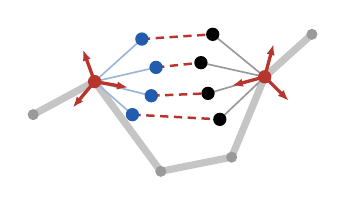
\begin{tikzpicture}[x=6mm, y=6mm] \ipapair
      \end{tikzpicture}\par}
    \end{column}
    \begin{column}{0.68\textwidth}
      \say{\bl{Query}-key \gn{distances} in global coordinates:}
      {$\big\|\Tg\circ \pu{T_i}\circ\bl{\vec{\mathbf q}_{ip}}-\Tg\circ \pu{T_j}\circ\vec{\mathbf k}_{jp}\big\| =\big\|\pu{T_i}\circ\bl{\vec{\mathbf q}_{ip}}-\pu{T_j}\circ\vec{\mathbf k}_{jp}\big\|$\par}
      \vspace{3mm}
      \say{Output points in \pu{frame} $i$, with $\textstyle\sum_j a_{ij}=1$:}
      {$(\Tg\circ \pu{T_i})^{-1}\circ\textstyle\sum_j a_{ij}\,\Tg\circ \pu{T_j}\circ\vec{\mathbf v}_{jp} = \pu{T_i}^{-1}\circ\textstyle\sum_j a_{ij}\,\pu{T_j}\circ\vec{\mathbf v}_{jp}$\par}
      \vspace{3mm}
      \say{\pu{Frame} update, composed in local coordinates:}
      {$(\Tg\circ \pu{T_i})\circ T_i^{\text{upd}} = \Tg\circ(\pu{T_i}\circ T_i^{\text{upd}})$\par}
    \end{column}
  \end{columns}
  \vspace{5mm}
  \key{The attention output is invariant. The frame update is equivariant.}
\end{frame}

\begin{frame}[t]{FAPE and Chirality}{SI 1.8.1 and 1.9.3, Algorithm 21, equations 11 to 17, Suppl.\ Fig.~9}
  % One row per step: the pictogram next to the sentence it illustrates.
  \begin{columns}[c,onlytextwidth]
    \begin{column}{0.42\textwidth}
      \centering\pictoatoms
    \end{column}
    \begin{column}{0.56\textwidth}
      \say{\pu{\textit{Frames}} from N, C$\alpha$, C by Gram--Schmidt.\\ Always right-handed: $\pu{\mathbf e_3}=\pu{\mathbf e_1}\times\pu{\mathbf e_2}$.}
    \end{column}
  \end{columns}
  \vspace{2mm}
  \begin{columns}[c,onlytextwidth]
    \begin{column}{0.42\textwidth}
      \centering\pictomirrorpage
    \end{column}
    \begin{column}{0.56\textwidth}
      \say{Mirroring flips the sign of $\bl{z}$ in each local \pu{frame}:}
      {$\mathrm{FAPE}(X,X_{\text{mirror}})=2\sum_{ki}\big|(\pu{T_k}^{-1}\circ\bl{\mathbf x_i})_{\bl{z}}\big|$\par}
    \end{column}
  \end{columns}
  \vspace{3mm}
  \say{With a distance-only loss (dRMSD), the model often predicts mirror images.}
  \key{FAPE penalises the mirror image of the true structure.}
\end{frame}

\begin{frame}[t]{Generalisation to New Structures}{\ck{JEP+21}, Fig.~2a and 2b, p.~585}
  % Each panel: a header saying what it measures and one line saying what it shows, all centred
  % in its column. Percentages read off the figure, the median from the caption.
  \say{Chains released after training. No template above 40\,\% identity.}
  \vspace{-1mm}
  \begin{columns}[T,onlytextwidth]
    \begin{column}{0.48\textwidth}
      \centering
      {\small\textbf{Backbone error per chain}\par}
      \vspace{1mm}
      \begin{marked}[25mm]{2}{39 631.8 465 49}
        \fill[cover] (0.015,0.91) rectangle (0.085,1.01);   % panel letter a
        \draw[ETHRed, line width=1pt, rounded corners=1pt] (0.806,0.215) rectangle (0.913,0.685);   % the chains above 8 A
      \end{marked}\par
      \vspace{1mm}
      {\small\raggedright Median 1.46\,\AA. {\color{ETHRed}17\,\% lie above 8\,\AA}. Some of these have misplaced domains.\par}
    \end{column}
    \begin{column}{0.48\textwidth}
      \centering
      {\small\textbf{Side chains against backbone}\par}
      \vspace{1mm}
      \begin{marked}[37mm]{2}{153.8 637.2 306 49}
        \fill[cover] (-0.01,0.92) rectangle (0.012,1.01);  % edge of panel letter b
        % the two ranges the sentence names: lDDT-Ca below 50 (red) and near 100 (green)
        \fill[ETHRed, opacity=0.13] (0.152,0.194) rectangle (0.46,0.957);
        \fill[CalloutGreen, opacity=0.16] (0.892,0.194) rectangle (0.95,0.957);
      \end{marked}\par
      \vspace{1mm}
      {\small\raggedright \gn{lDDT-C$\alpha$ near 100}: 93\,\% of side-chain angles $\chi_1$ correct. {\color{ETHRed}Below 50}: about 55\,\%.\par}
    \end{column}
  \end{columns}
  \vspace{2mm}
  \key{High accuracy on chains released after training.}
  \reffootnote{3,144 and 5,317 chains. Percentages read off the figure. A $\chi_1$ angle counts as correct within 40\textdegree}
\end{frame}

\begin{frame}[t]{Reported Failures of AlphaFold 3}{\ck{AAD+24}, Fig.~5b and 5e, p.~497 and 499}
  % colours sampled from the paper's figures, the orange darkened for legibility as text
  \definecolor{AFthreeOrange}{RGB}{222,140,10}\definecolor{AFthreeBlue}{RGB}{60,140,175}\definecolor{AFthreePink}{RGB}{175,64,118}
  % The two stereochemistry failures the AF3 paper reports (p. 497). Left: chirality, our constraint 3,
  % built into AlphaFold 2 by FAPE. Right: clashes, not one of our constraints.
  \vspace{2mm}
  \begin{columns}[T,onlytextwidth]
    \begin{column}{0.455\textwidth}
      \centering
      {\small\textbf{Wrong chirality}\par}
      \vspace{1mm}
      \begin{markedAFthree}[0.791\linewidth]{2}{308 645 112 48}
        \fill[cover] (0,0.85) rectangle (0.09,1.01);
      \end{markedAFthree}\par
      \vspace{1mm}
      {\small\raggedright {\color{AFthreeOrange}Predicted alpha form}, {\color{ETHGray}true beta form}.\\ Wrong in 4.4\,\% of predictions.\par}
    \end{column}
    \begin{column}{0.455\textwidth}
      \centering
      {\small\textbf{Overlapping chains}\par}
      \vspace{1mm}
      \begin{markedAFthree}[0.591\linewidth]{2}{352 376 115 318}
        \fill[cover] (0,0.85) rectangle (0.09,1.01);
      \end{markedAFthree}\par
      \vspace{1mm}
      {\small\raggedright {\color{AFthreeBlue}Protein} and {\color{AFthreePink}DNA} overlap.\\ Mostly in large complexes.\par}
    \end{column}
  \end{columns}
  \vspace{1mm}
  \key{Penalties in sample ranking reduce both failures.}
  \reffootnote{PDB 7CTM and 7PEU. The 4.4\,\% is on the PoseBusters benchmark}
\end{frame}

\end{document}
